%%%%%%%%%%%%%%%%%%%%%%%%%%%%%%%%%%%%%%%%%
% Beamer Presentation
% LaTeX Template
% Version 1.0 (10/11/12)
%
% This template has been downloaded from:
% http://www.LaTeXTemplates.com
%
% License:
% CC BY-NC-SA 3.0 (http://creativecommons.org/licenses/by-nc-sa/3.0/)
%
%%%%%%%%%%%%%%%%%%%%%%%%%%%%%%%%%%%%%%%%%

%----------------------------------------------------------------------------------------
%	PACKAGES AND THEMES
%----------------------------------------------------------------------------------------

\documentclass{beamer}

\mode<presentation> {

% The Beamer class comes with a number of default slide themes
% which change the colors and layouts of slides. Below this is a list
% of all the themes, uncomment each in turn to see what they look like.

%\usetheme{default}
%\usetheme{AnnArbor}
%\usetheme{Antibes}
%\usetheme{Bergen}
%\usetheme{Berkeley}
%\usetheme{Berlin}
%\usetheme{Boadilla}
%\usetheme{CambridgeUS}
%\usetheme{Copenhagen}
%\usetheme{Darmstadt}
%\usetheme{Dresden}
%\usetheme{Frankfurt}
%\usetheme{Goettingen}
%\usetheme{Hannover}
%\usetheme{Ilmenau}
%\usetheme{JuanLesPins}
%\usetheme{Luebeck}
\usepackage[francais]{babel}
\usetheme{Madrid}
\usepackage[utf8]{inputenc}  
\usepackage[T1]{fontenc}
%\usetheme{Malmoe}
%\usetheme{Marburg}
%\usetheme{Montpellier}
%\usetheme{PaloAlto}
%\usetheme{Pittsburgh}
%\usetheme{Rochester}
%\usetheme{Singapore}
%\usetheme{Szeged}
%\usetheme{Warsaw}

% As well as themes, the Beamer class has a number of color themes
% for any slide theme. Uncomment each of these in turn to see how it
% changes the colors of your current slide theme.

%\usecolortheme{albatross}
%\usecolortheme{beaver}
%\usecolortheme{beetle}
%\usecolortheme{crane}
%\usecolortheme{dolphin}
%\usecolortheme{dove}
%\usecolortheme{fly}
%\usecolortheme{lily}
%\usecolortheme{orchid}
%\usecolortheme{rose}
%\usecolortheme{seagull}
%\usecolortheme{seahorse}
%\usecolortheme{whale}
%\usecolortheme{wolverine}

%\setbeamertemplate{footline} % To remove the footer line in all slides uncomment this line
%\setbeamertemplate{footline}[page number] % To replace the footer line in all slides with a simple slide count uncomment this line

%\setbeamertemplate{navigation symbols}{} % To remove the navigation symbols from the bottom of all slides uncomment this line
}

\usepackage{graphicx} % Allows including images
\usepackage{booktabs} % Allows the use of \toprule, \midrule and \bottomrule in tables

%----------------------------------------------------------------------------------------
%	TITLE PAGE
%----------------------------------------------------------------------------------------

\title[Stage de Fin d'Études]{Intégration d'un dispositif de communication en champ proche (NFC) au Géocube} % The short title appears at the bottom of every slide, the full title is only on the title page

\author{Mohamed-Amjad LASRI} % Your name
\institute[IT3 - GTSI] % Your institution as it will appear on the bottom of every slide, may be shorthand to save space
{
École Nationale des Sciences Géographiques \\ % Your institution for the title page
\medskip
\textit{mohamed-amjad.lasri@ensg.eu} % Your email address
}
\date{\today} % Date, can be changed to a custom date

\begin{document}

\begin{frame}
\titlepage % Print the title page as the first slide
\end{frame}

\begin{frame}
\frametitle{Sommaire} % Table of contents slide, comment this block out to remove it
\tableofcontents % Throughout your presentation, if you choose to use \section{} and \subsection{} commands, these will automatically be printed on this slide as an overview of your presentation
\end{frame}

%----------------------------------------------------------------------------------------
%	PRESENTATION SLIDES
%----------------------------------------------------------------------------------------

%------------------------------------------------
\section{Le système Géocube:} % Sections can be created in order to organize your presentation into discrete blocks, all sections and subsections are automatically printed in the table of contents as an overview of the talk
%------------------------------------------------
\begin{frame}
\frametitle{Le système Géocube}
\begin{itemize}
\item Conçu par LOEMI-IGN et industrialisé par Kylia;
\item Réseau de capteurs pour mesurer les déformations avec une précision millimétrique;
\item Ultra basse consommation électrique;
\item Adapté à la surveillance environnementale en temps de crise;
\item Doté d'un noyau temps-réel dur développé à LOEMI-IGN.
\end{itemize}
\end{frame}

%------------------------------------------------

\begin{frame}
\frametitle{Le système Géocube:}
\begin{figure}
\centering
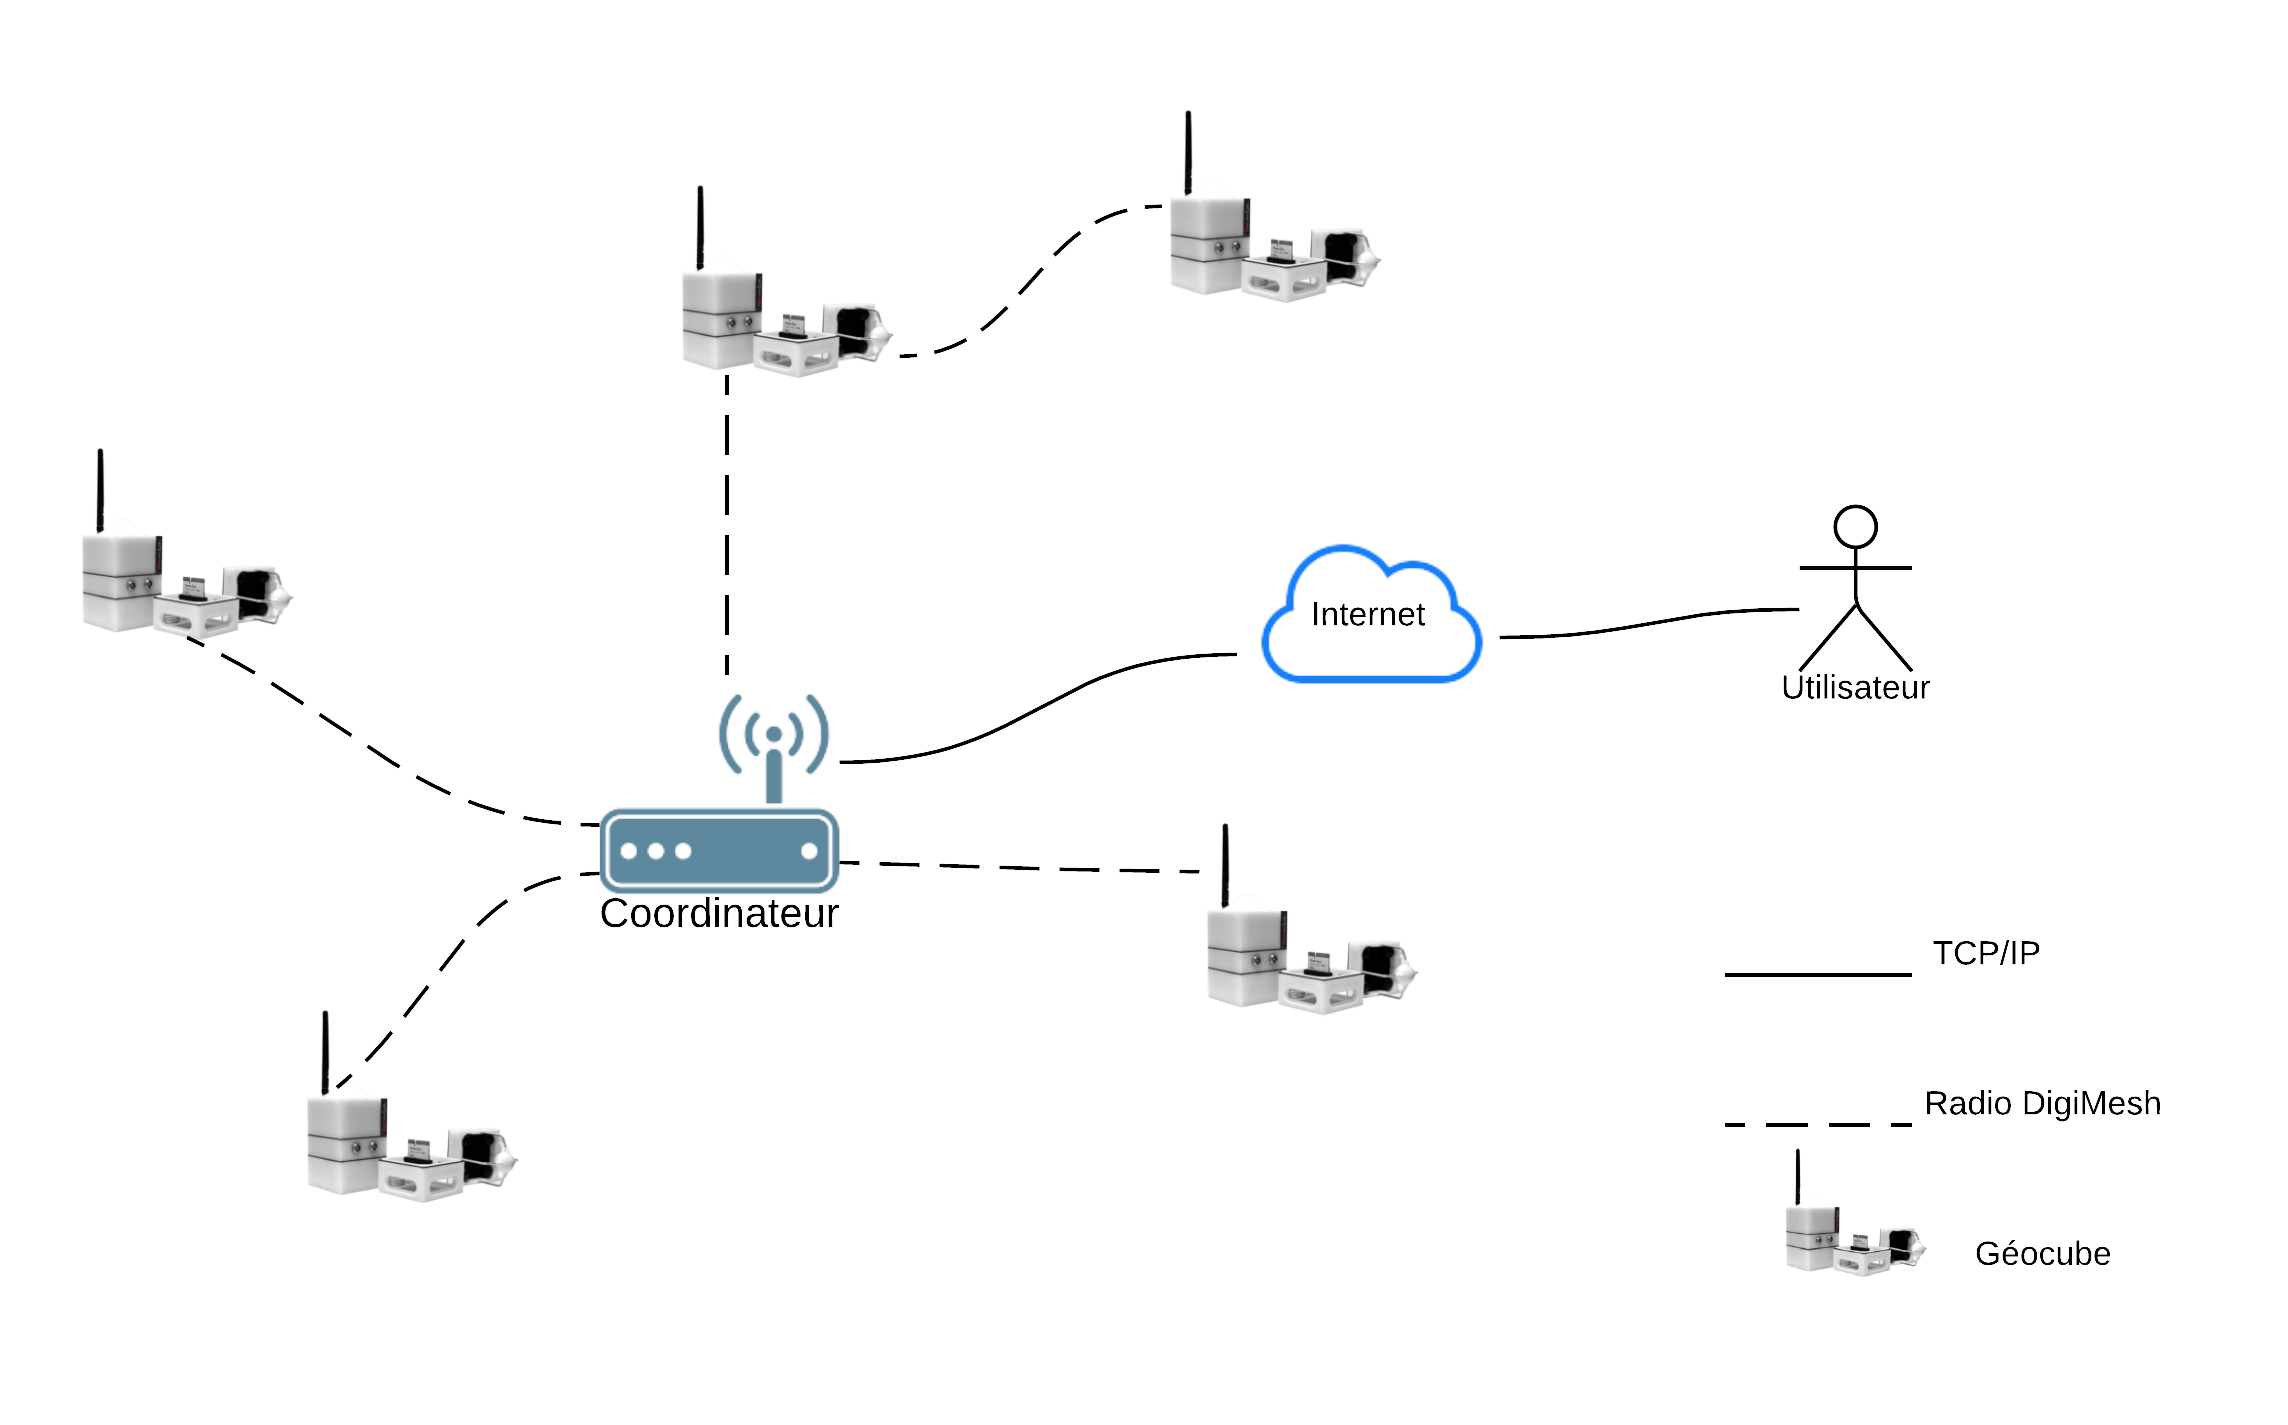
\includegraphics[scale=0.53]{images/grid.png}
\label{fig:grid}
\caption{Réseau de Géocubes}
\end{figure}
\end{frame}

%------------------------------------------------
\begin{frame}
\frametitle{Le système Géocube}
On peut communiquer avec un Géocube:
\begin{itemize}
\item en envoyant des commandes par radio depuis le coordinateur.
\item lien filaire: port série (Par souci d'étanchéité du boîtier, cette solution n'est pas maintenu dans la version industrielle).
\end{itemize}

Ajouter un autre moyen de communication:
\begin{itemize}
\item La communication en champ proche (NFC)
\end{itemize}
\begin{figure}
\centering

\includegraphics[scale=0.7]{images/g3nfc.png}
\end{figure}
\end{frame}

%------------------------------------------------

\section{Intégration d'une solution NFC au Géocube}

%------------------------------------------------
\begin{frame}
\frametitle{La communication en champ proche (NFC)}
\begin{itemize}
\item Technologie utilisée principalement pour identifier les objets et échanger des information peu volumineuse;
\item Opérant en 13.56Mhz, la distance entre les dispositifs ne doit pas dépasser 3cm;
\item Des dizaines de normes pour standardiser les protocoles de communication;
\end{itemize}
Deux modes de communication:
\begin{itemize}
\item Card emulation;
\item Peer2Peer.
\end{itemize}
\end{frame}

%------------------------------------------------
\subsection{Choix de la puce NFC}
\begin{frame}
\frametitle{Choix de la puce NFC}
La plupart des puces existant sur le marché sont en mode "Card emulation". Quelques constructeurs proposent des puces P2P:

\begin{table}
\centering
\resizebox{\columnwidth}{!}{
\begin{tabular}{|c|c|c|c|c|c|c|c|}
\hline
Référence & Constructeur & Prix(\$) & Débit(kbps) & ISO 14443 & Interface & T(deg) & RAM\\ \hline
TRF7970A & TI & 6.98 & 424 & 3 & SPI-Paral & -40 - 110 & NC\\
RF430CL330H & TI & 1.74 & 848 & 3 & SPI-I2C & -40 - 85 & 3KO\\
AS3953 & AMS & 1.09 & 848 & 3 & SPI & -40 - 85 & NC\\
PN533 & NXP & NC & 848 & 3 & USB2 & -40 - 125 & 1KO\\
\hline
\end{tabular}
}
\end{table}

Maintient de l'AS3953:
\begin{itemize}
\item Modification de la carte Géocube actuelle
\item Basse consommation électrique
\end{itemize}

\end{frame}

%------------------------------------------------
\subsection{Développement de l'antenne}
% Schéma electrique d'une antenne

\begin{frame}

Le circuit puce NFC+Antenne peut être assimiler au circuit suivant.
\begin{figure}
\centering
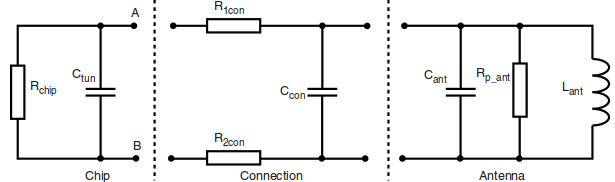
\includegraphics[scale=0.4]{images/withPARA.png}
\end{figure}

En calculant les R, C équivalents:
\begin{figure}
\centering
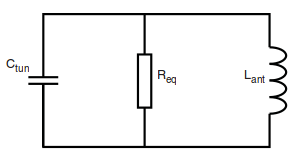
\includegraphics[scale=0.4]{images/circuiteq.png}
\end{figure}
\end{frame}

%------------------------------------------------
% Les trucs que j'ai essayé et l'antenne que j'ai fabriqué

\begin{frame}

Échantillons du commerce essayés:
\begin{figure}
\centering
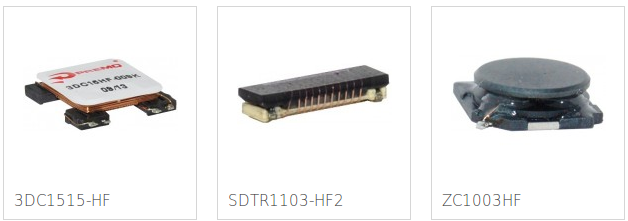
\includegraphics[scale=0.5]{images/antennas.png}
\end{figure}
\begin{itemize}
\item conception de quelques antennes artisanales;
\item impression des circuits électroniques correspondants;
\item expérimentation, ...
\end{itemize}
\end{frame}
%------------------------------------------------
% équations électriques

%------------------------------------------------
% Mode opératoire
\begin{frame}
\frametitle{Mode opératoire}
\begin{figure}
\centering
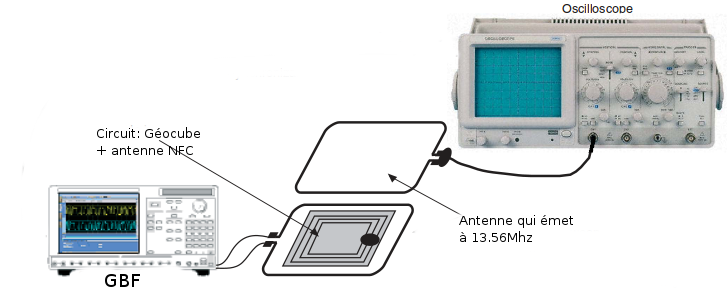
\includegraphics[scale=0.4]{images/gbfoscillo.png}
\end{figure}
\end{frame}
%------------------------------------------------
\subsection{Conception et développement des couches logicielles}
%------------------------------------------------
% communication global
\begin{frame}
\frametitle{Schéma des composants}
\begin{figure}
\centering
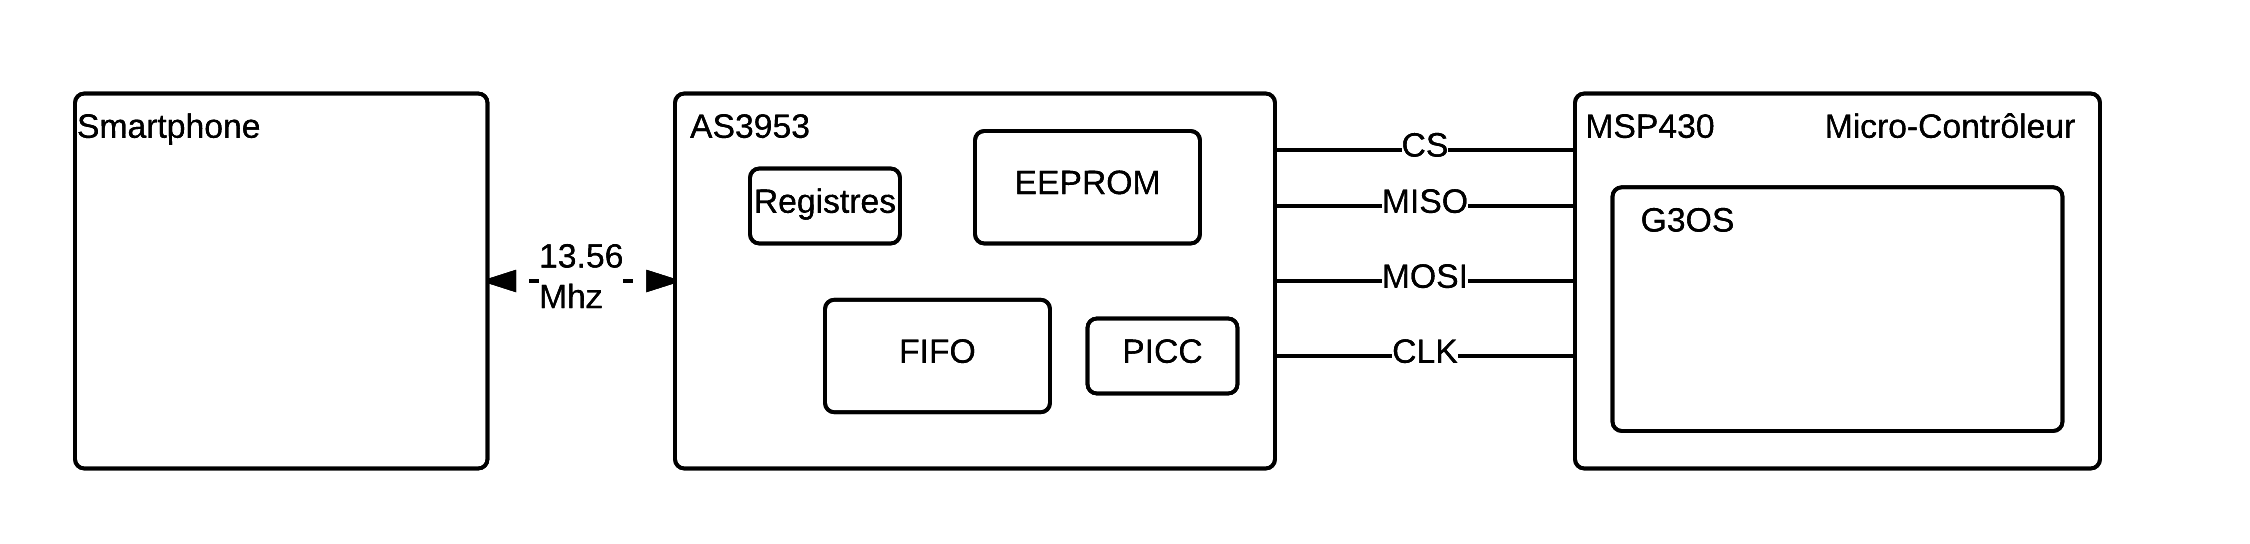
\includegraphics[scale=0.5]{images/block-diagram.png}
\end{figure}
\begin{itemize}
\item EEPROM: Electrically Erasable Programmable Read-Only Memory, 32 mots d'un 1octet chacun
\item PICC: Proximity Inductive Coupling Card, composant qui encapsule toute la logique liée aux 3 premiers niveaux de l'ISO/IEC14443 
\end{itemize}

\end{frame}
%------------------------------------------------
% communication global
\begin{frame}
\frametitle{Communication micro-contrôleur/Puce NFC}
\begin{figure}
\centering
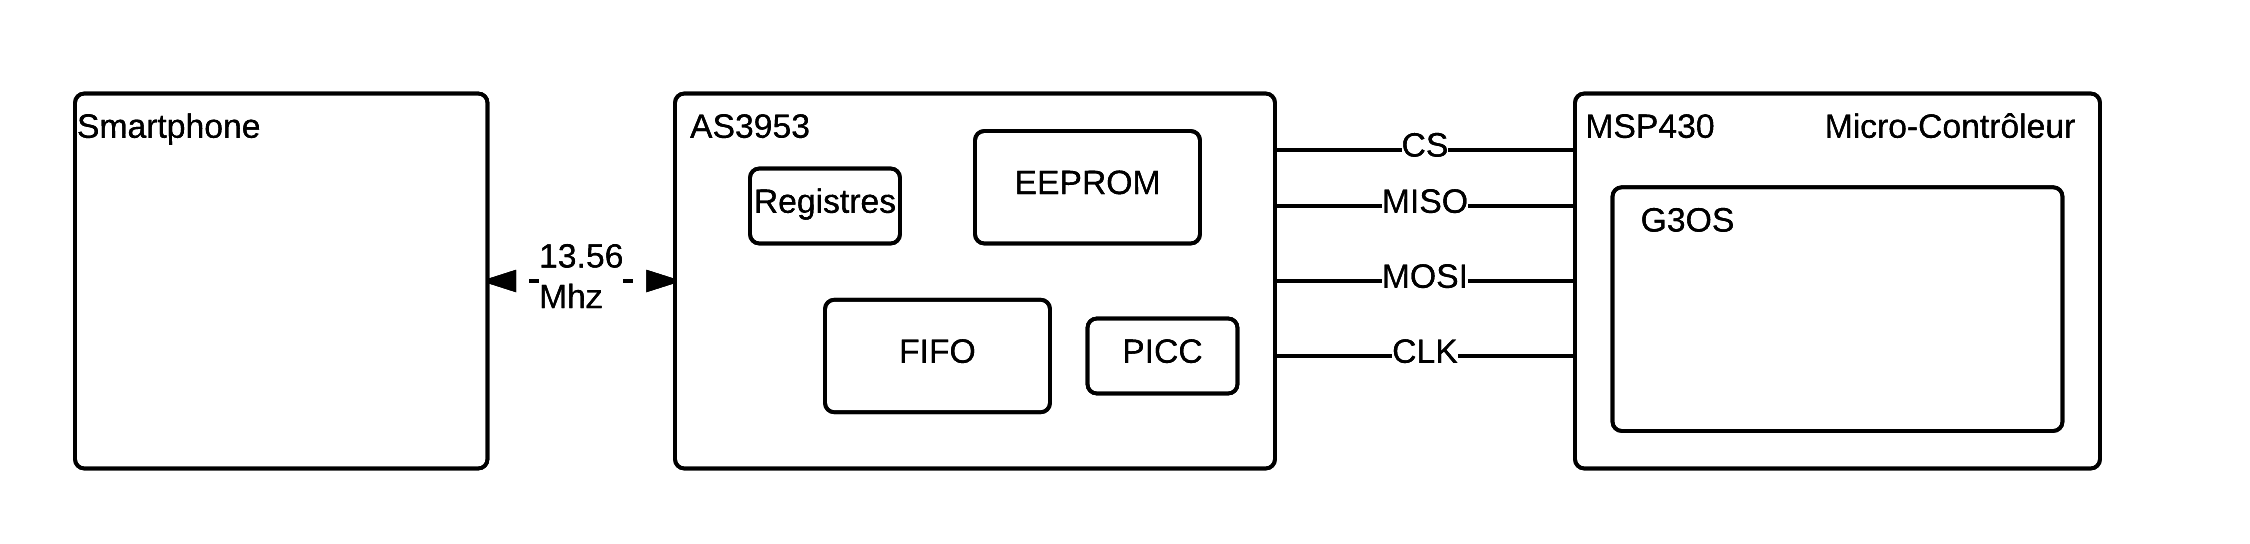
\includegraphics[scale=0.5]{images/block-diagram.png}
\end{figure}
Exemple: Écrire un mot dans la FIFO
\begin{itemize}
\item Le micro-contrôleur active le CS, la synchronisation de l'horloge du micro-contrôleur avec celle de la puce NFC est effectuée.
\item Le micro-contrôleur envoie 3 octets à travers le MOSI: Le premier correspond au mode de communication (1000 0000 pour écrire dans la FIFO), Le deuxième c'est l'adresse du mot qu'on veut écrire(0000 0000 pour écrire dans le premier mot) et l'octet qu'on veut écrire (1111 1111 par exemple). 1000 0000 0000 0000 1111 1111.
\item De même pour la lecture...

\end{itemize}

\end{frame}
%------------------------------------------------
% dire que n inclut pas le 4eme niveau est

\begin{frame}

Pour pouvoir communiquer avec un smartphone Android en mode P2P il faut implémenter le 4ème niveau de la norme ISO/IEC 14443.

Ce niveau n'est pas disponible par défaut dans la puce NFC choisie.

Le BTP (Block Transmission Protocol), définit un format de block d'échange comme suit:
\begin{tabular}[hf]{|c|c|c|c|c|c|c|c|}
\hline
\multicolumn{3}{|c|}{Prologue} & \multicolumn{3}{c|}{Information} & \multicolumn{2}{c|}{Epilogue} \\
\hline
PCB & [CID] & [NAD] & \multicolumn{3}{|c|}{[INF]} & \multicolumn{2}{c|}{EDC}\\
\hline
1 octet & 1 octet & 1 octet & \multicolumn{3}{|c|}{} & \multicolumn{2}{c|}{2 octets}\\
\hline
\end{tabular}
\end{frame}
%------------------------------------------------
% dire que n inclut pas le 4eme niveau est
\begin{frame}
\frametitle{PCB}
Le PCB(Protocol Control Byte), peut être un de ces trois octets:
\begin{itemize}
\item I-Block utilisé pour indiquer au dispositif destinataire que le bloc envoyé est
un bloc d’information et contient des octets dans le champs INF.
\item R-Block: utilisé pour indiquer une reconnaissance négative ou positive. Un R-
Block ne contient jamais de champs INF.
\item S-Block: utilisé pour échanger des informations de control entre le PCD et le
PICC. Il existe deux types de S-Block : le DESELECT qui n’est jamais suivit par un
champ INF et le WTE qui doit être suivit par un octets dans le champ INF.
\end{itemize}
\end{frame}

%------------------------------------------------
% dire que n inclut pas le 4eme niveau est
\begin{frame}
\frametitle{Réception d'un bloc}
L'échange des blocs en NFC est toujours initié par le smartphone.

Pour recevoir un bloc du smartphone:
\begin{itemize}
\item Le micro-contrôleur reçoit un signal d'interruption de la puce NFC;
\item acquitte l'interruption;
\item lance la tâche NFC;
\item la tâche NFC commence par lire le registre d'erreurs, pour voir est ce que le bloc envoyé a passé les 3 premiers niveaux de l'ISO/IEC 14443 sans problèmes;
\item la tâche NFC lit le registre principal des interruptions pour vérifier qu'elle a été lancée suite à une activation par un autre dispositif qui supporte l'ISO/IEC 14443;
\item la tâche NFC lit la file FIFO de la puce NFC, Le premier mot est soit un R-Block, I-Block ou S-Block.
\end{itemize}

\end{frame}

%------------------------------------------------
% dire que n inclut pas le 4eme niveau est
\begin{frame}
\frametitle{Envoi d'un bloc}
Pour envoyer un bloc du Géocube au smartphone:
\begin{itemize}
\item La tâche NFC écrit dans la FIFO le bloc qu'elle veut envoyée;
\item Elle envoie ensuite une commande direct au PICC pour lui demander de transférer les octets de la FIFO au smartphone.
\item La réponse à un bloc envoyé par le smartphone doit être effectuée dans un délais bien déterminé.

\begin{figure}
\centering
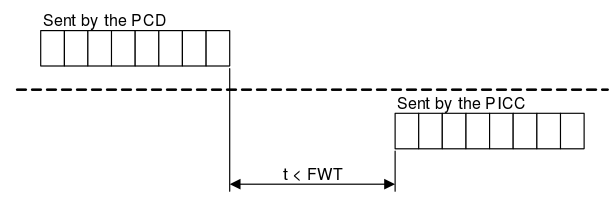
\includegraphics[scale=0.45]{images/fwt.png}
\end{figure}

\end{itemize}
\end{frame}

%------------------------------------------------
% picc check
\begin{frame}
\frametitle{HandShake NFC}
\begin{figure}
\centering
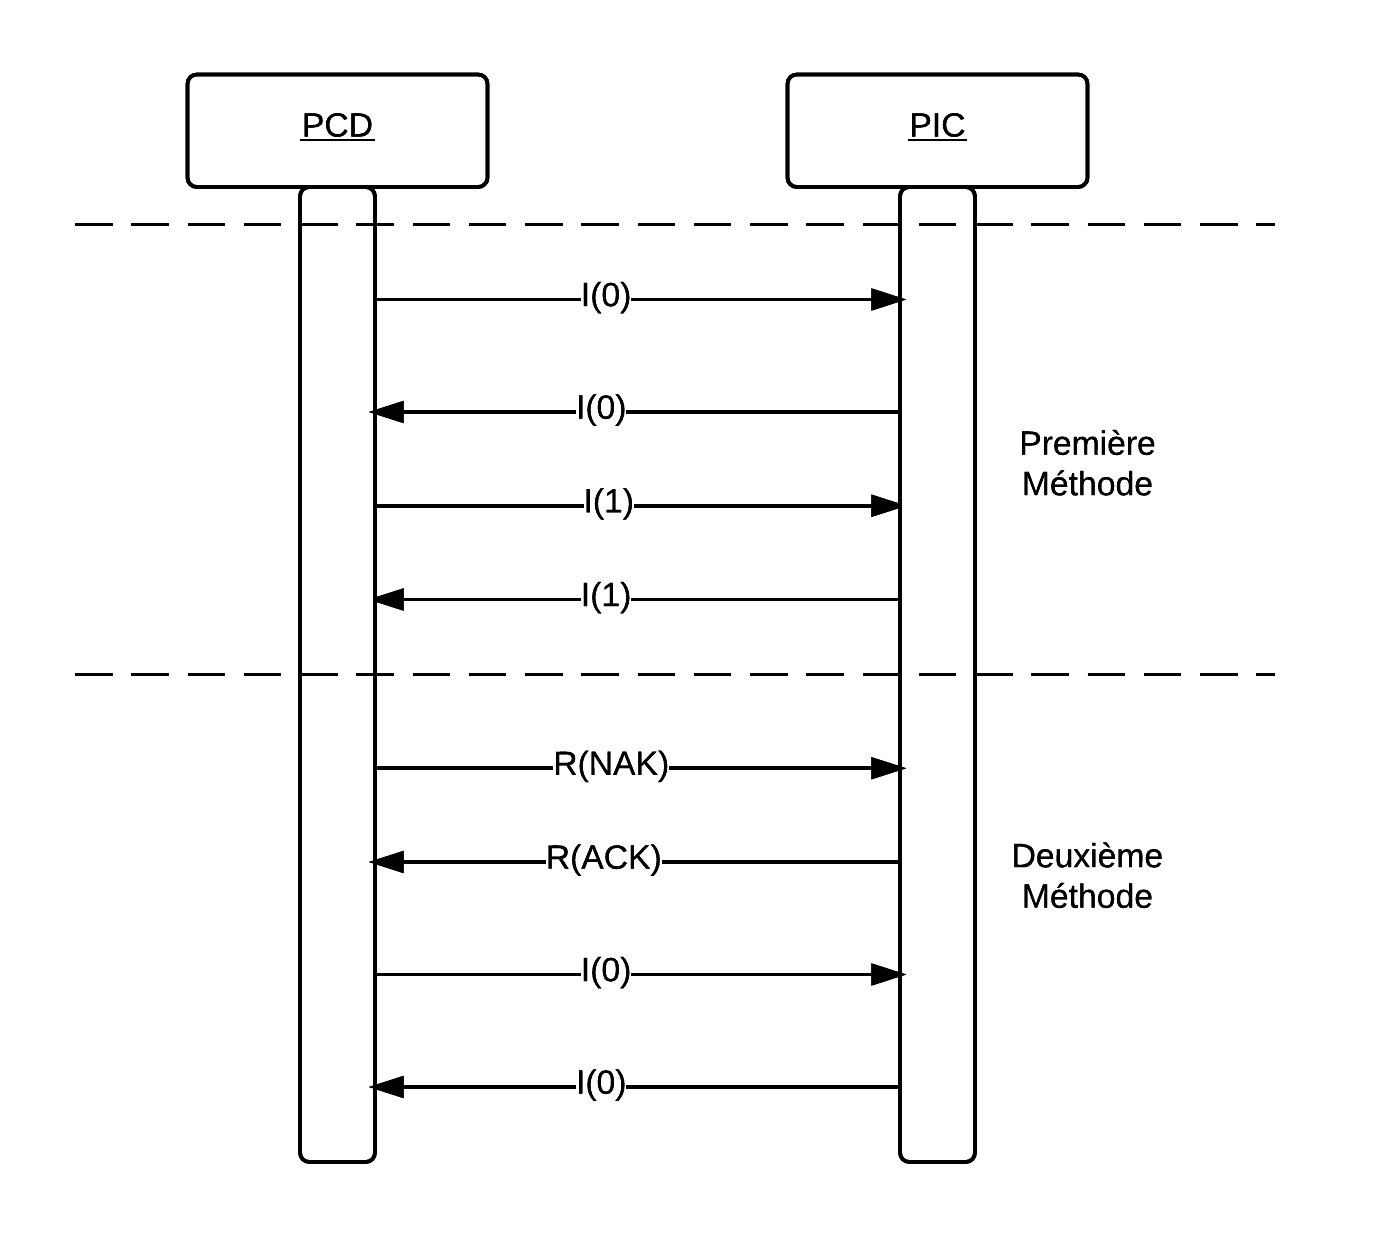
\includegraphics[scale=0.5]{images/presencecheck.png}
\end{figure}

Lors du HandShake la tâche NFC envoie dans le premier I-Block échangé, l'URI de l'application Android qu'elle veut lancer
\end{frame}

%------------------------------------------------
% picc check
\begin{frame}
\frametitle{Transfert des blocs}
\begin{figure}
\centering
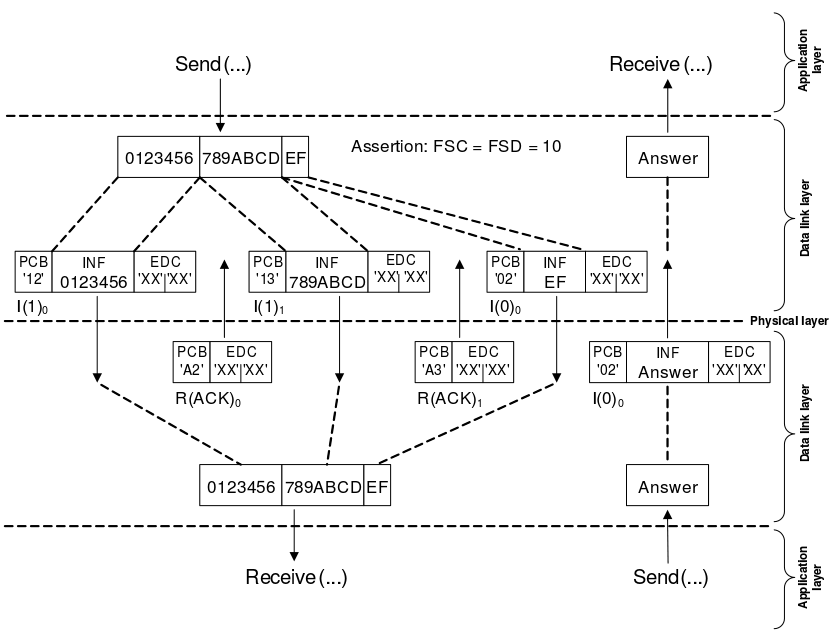
\includegraphics[scale=0.25]{images/chaining.png}
\end{figure}
Les mots envoyés par la tâche NFC: 1111 1XXX | 0101 0101 0101 0101 |
\end{frame}

%------------------------------------------------
% picc check
\begin{frame}
\frametitle{Deselect}
\begin{figure}
\centering
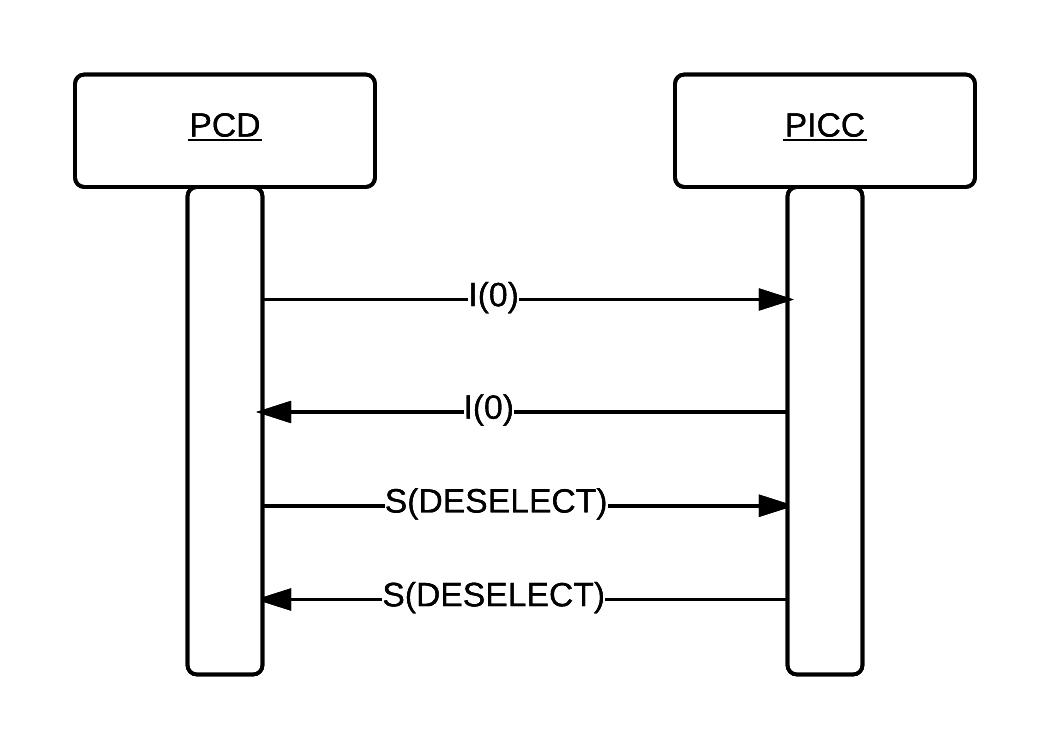
\includegraphics[scale=0.5]{images/deselect.png}
\end{figure}
Fin de la transmission...
\end{frame}

%------------------------------------------------
\subsection{Conception et développement de l'application Android}
%------------------------------------------------
\begin{frame}
\frametitle{Foreground dispatch system}
\begin{itemize}
\item L'application G3NFC doit se lancer automatiquement lorsqu'un Géocube est scanné.
\item Utiliser le foreground dispatch system d'android
\end{itemize}
\begin{figure}
\centering
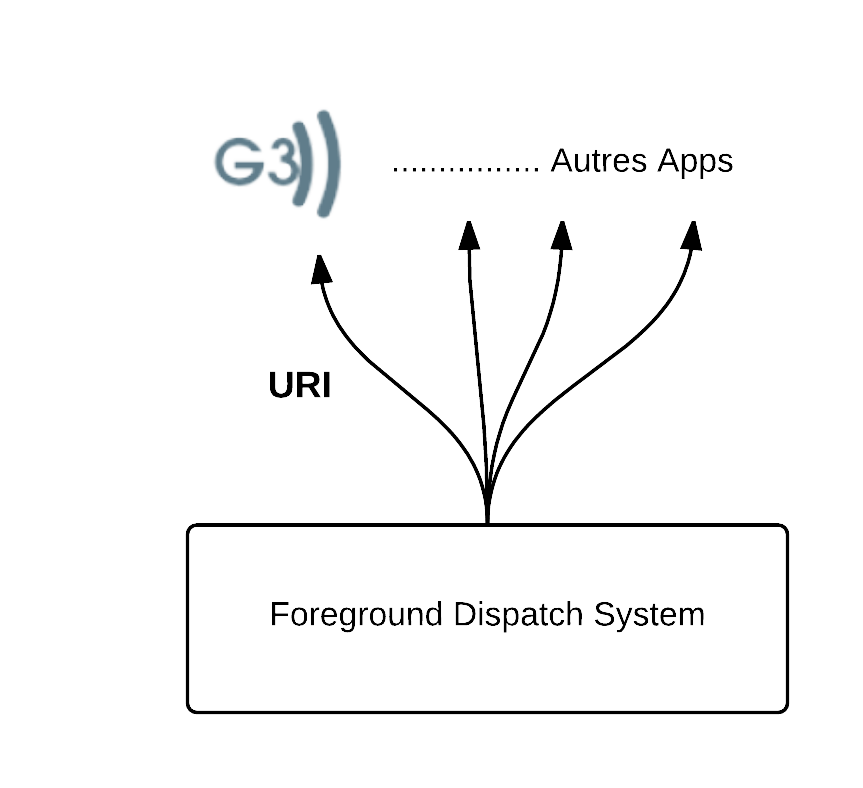
\includegraphics[scale=0.6]{images/foreground.png}

\end{figure}
\end{frame}

\section{Conception, Développement et déploiement d'un système de mise à jour pour le coordinateur des Géocubes}
\subsection{Analyse du besoin}
%------------------------------------------------
\begin{frame}
\frametitle{Contexte générale}
\begin{figure}
\centering
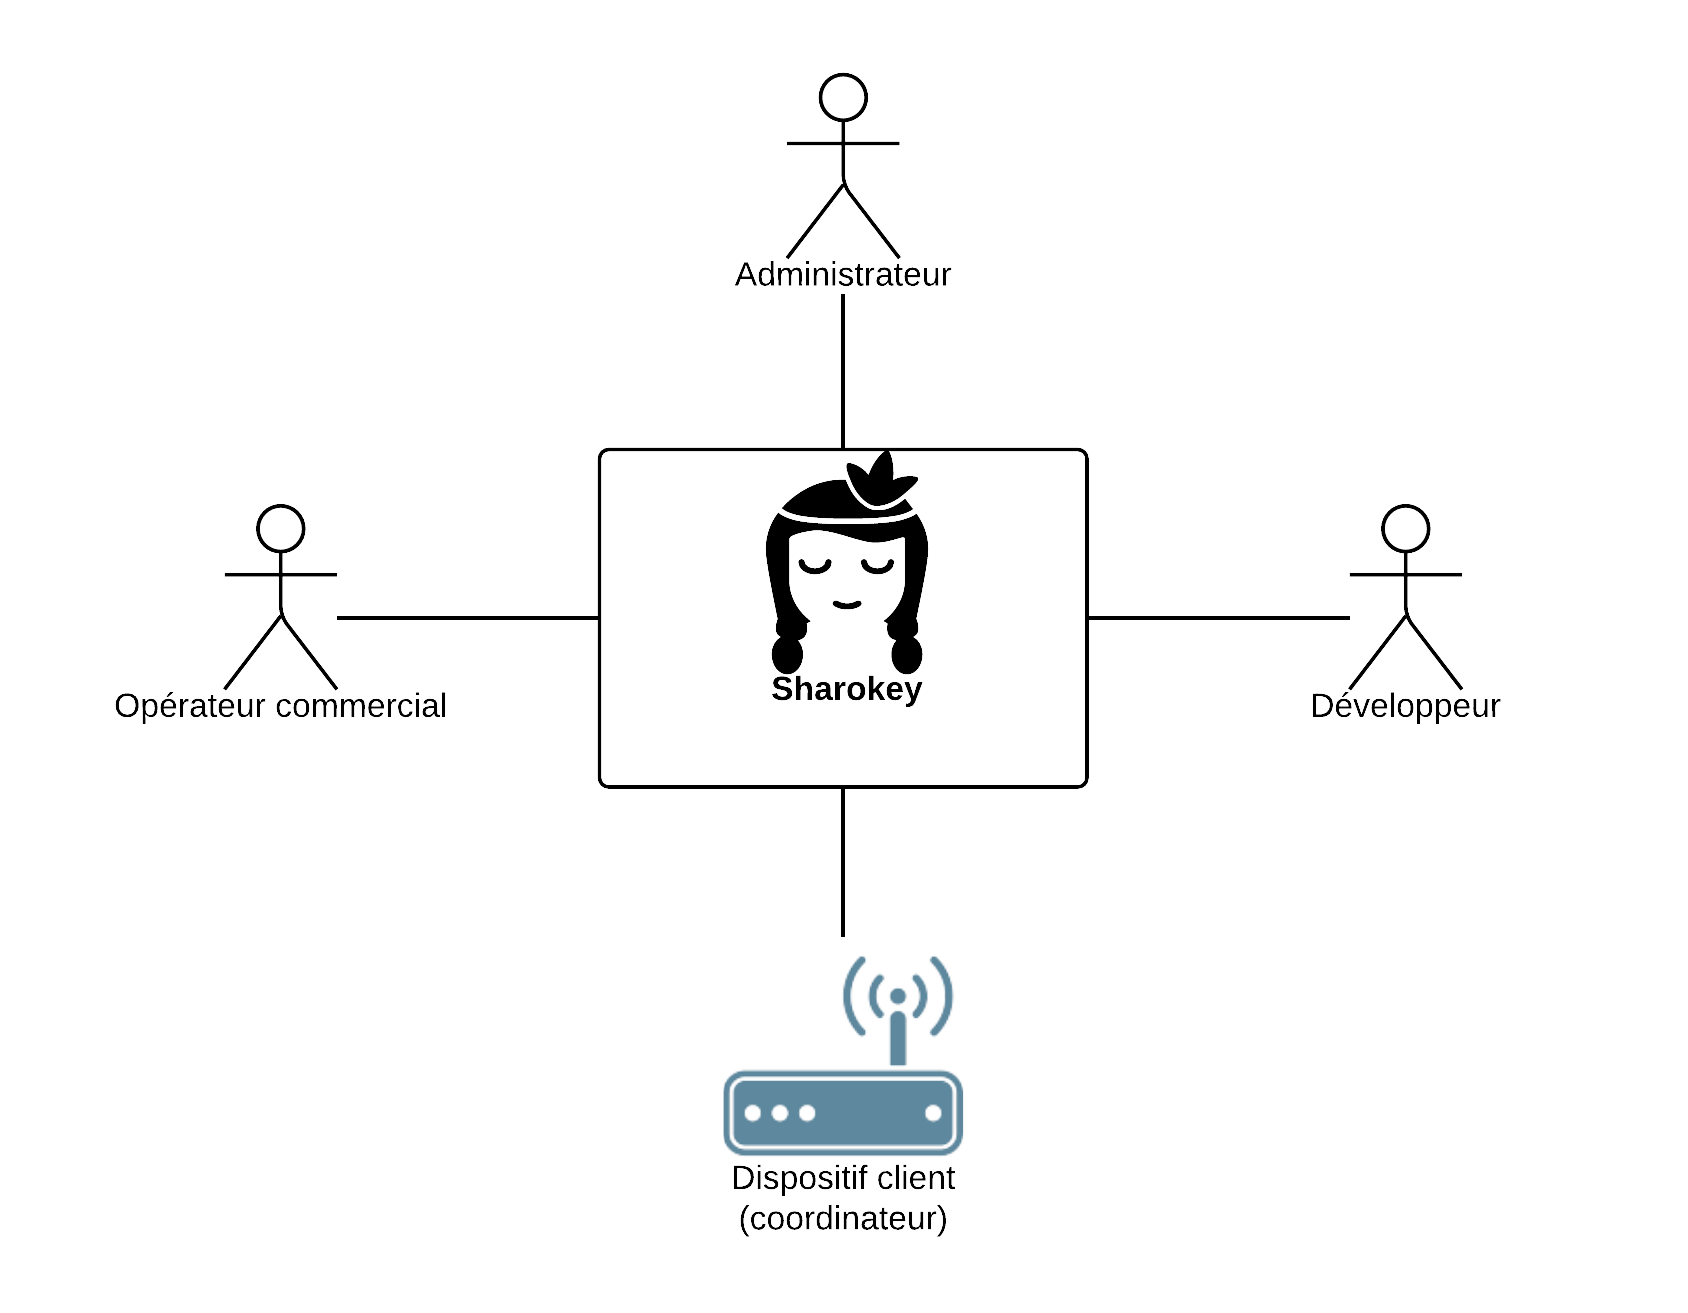
\includegraphics[scale=0.7]{images/context_general.png}
\end{figure}
\end{frame}
%------------------------------------------------
\subsection{Conception statique}
\begin{frame}
\frametitle{Cas d'utilisation}
\begin{figure}
\centering
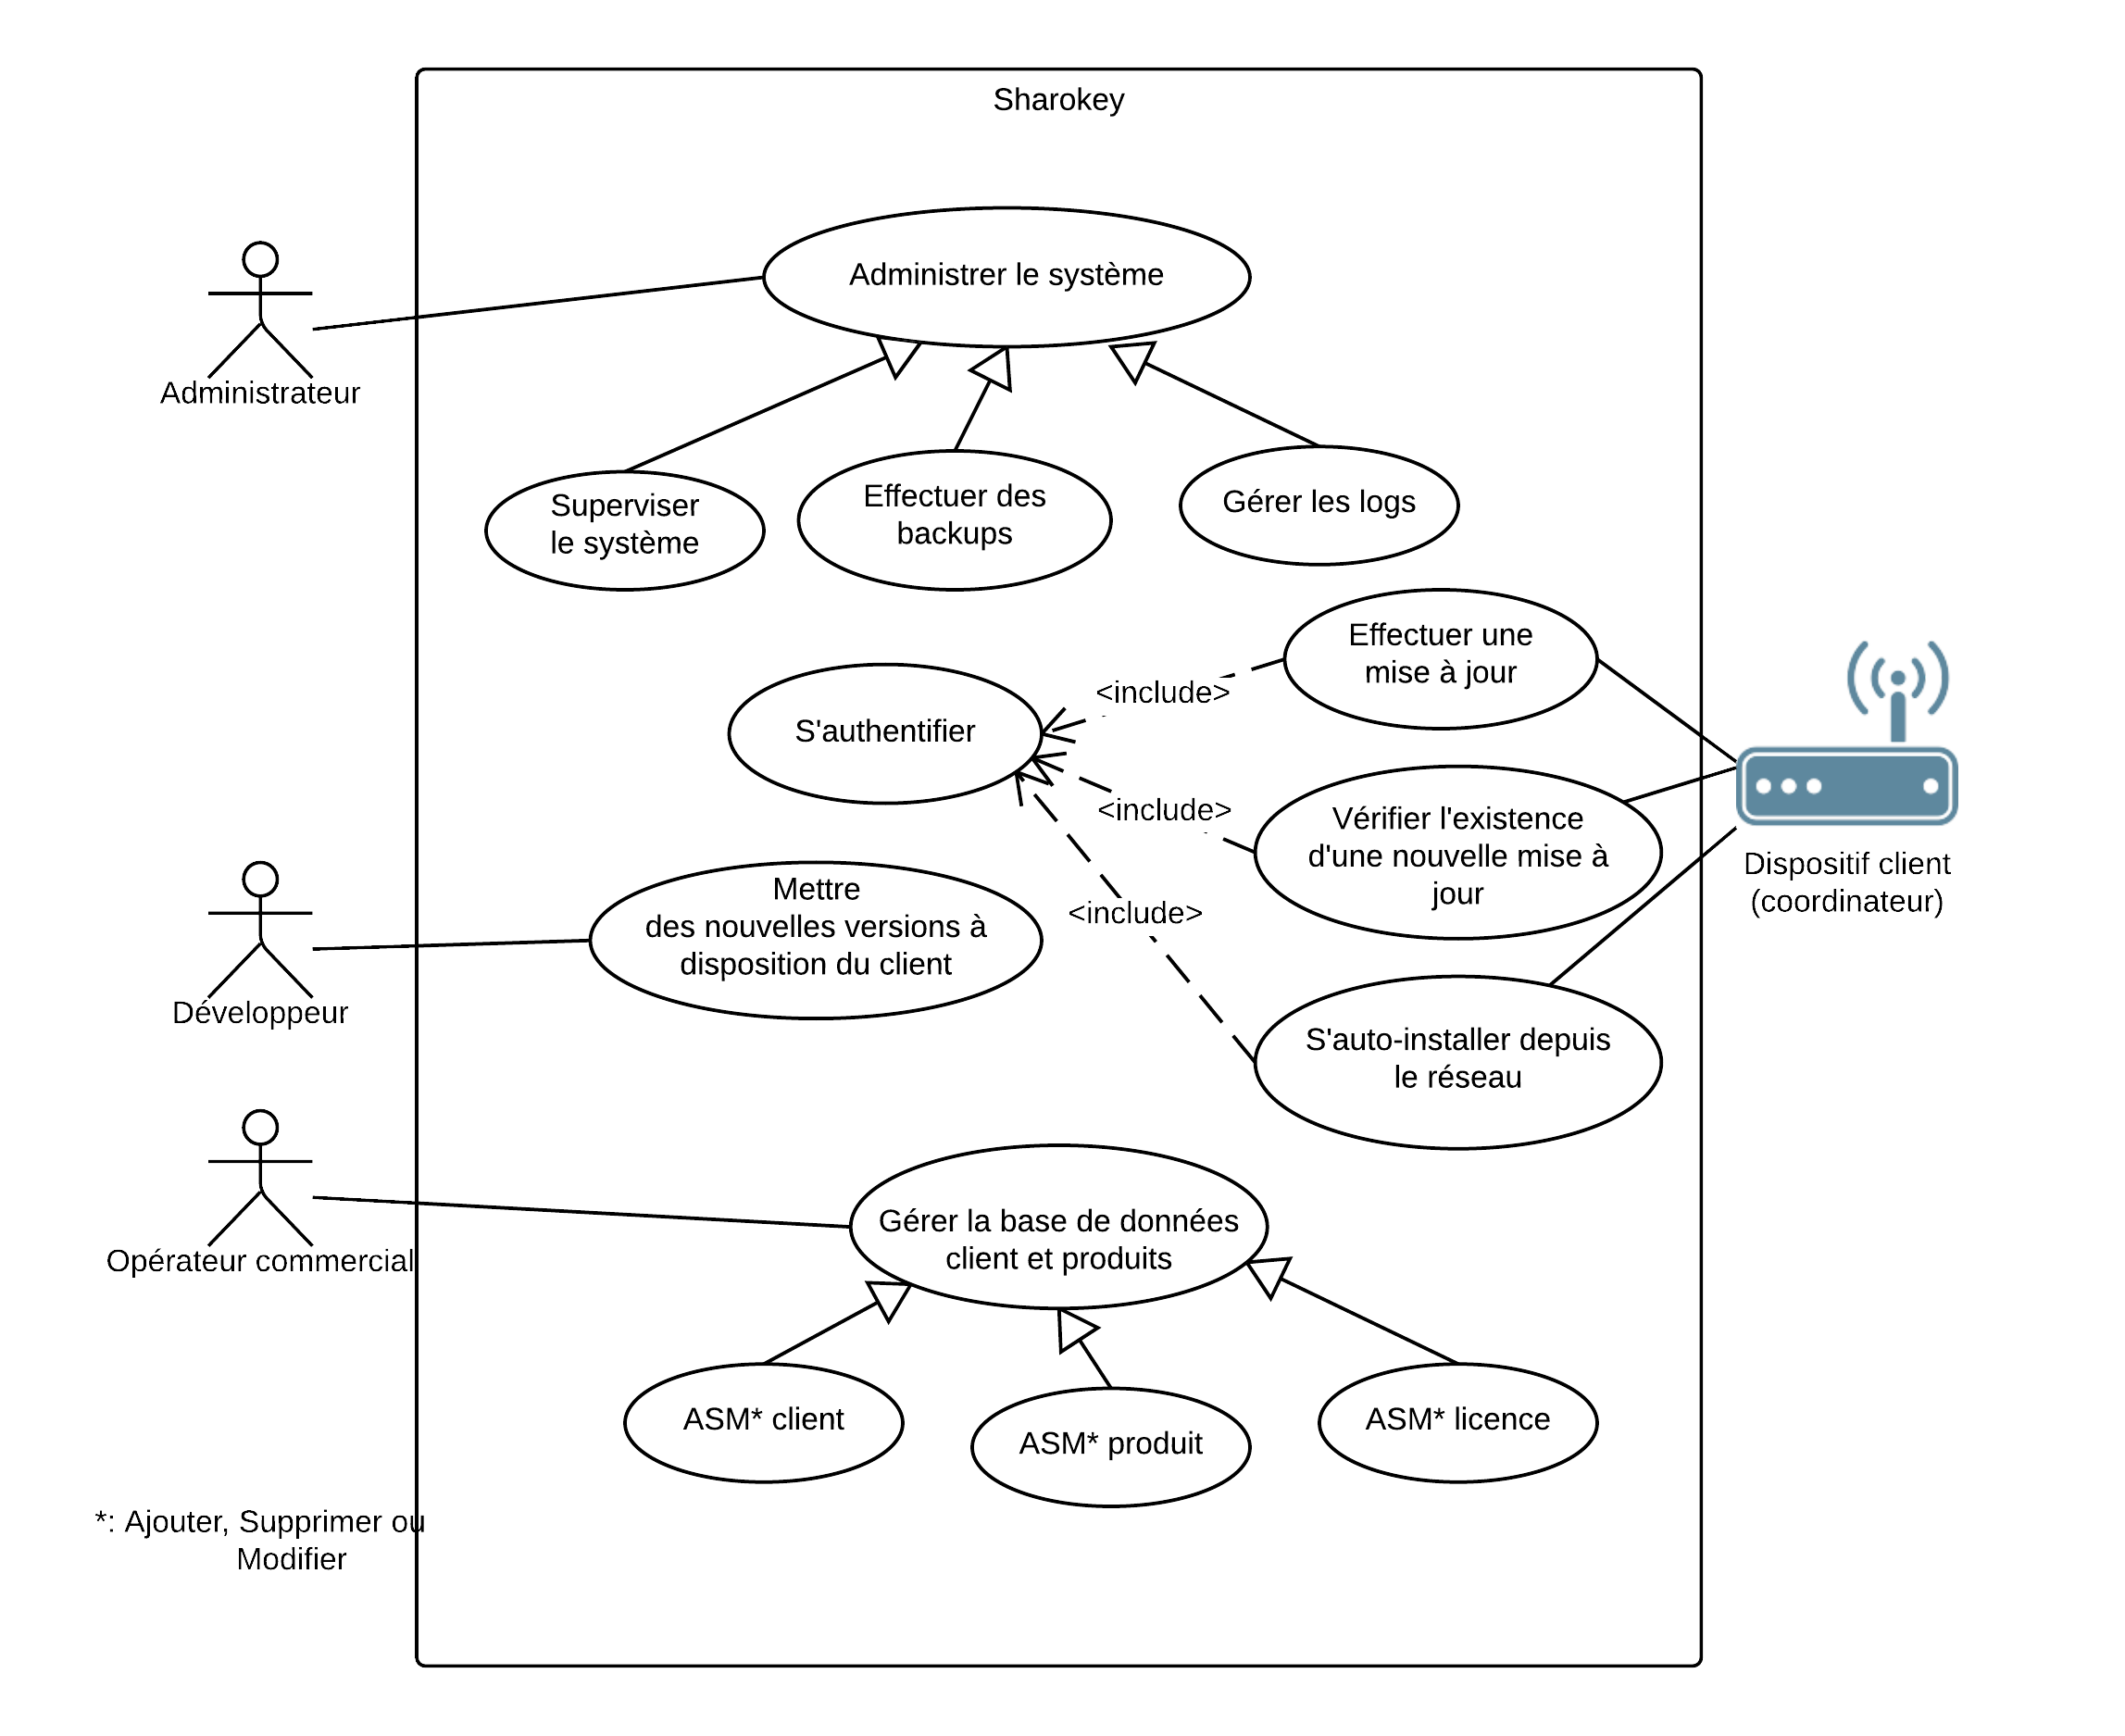
\includegraphics[scale=0.45]{images/use_case_sharokey.png}
\end{figure}
\end{frame}

\begin{frame}
\frametitle{Modèle Physique des Données}
\begin{figure}
\centering
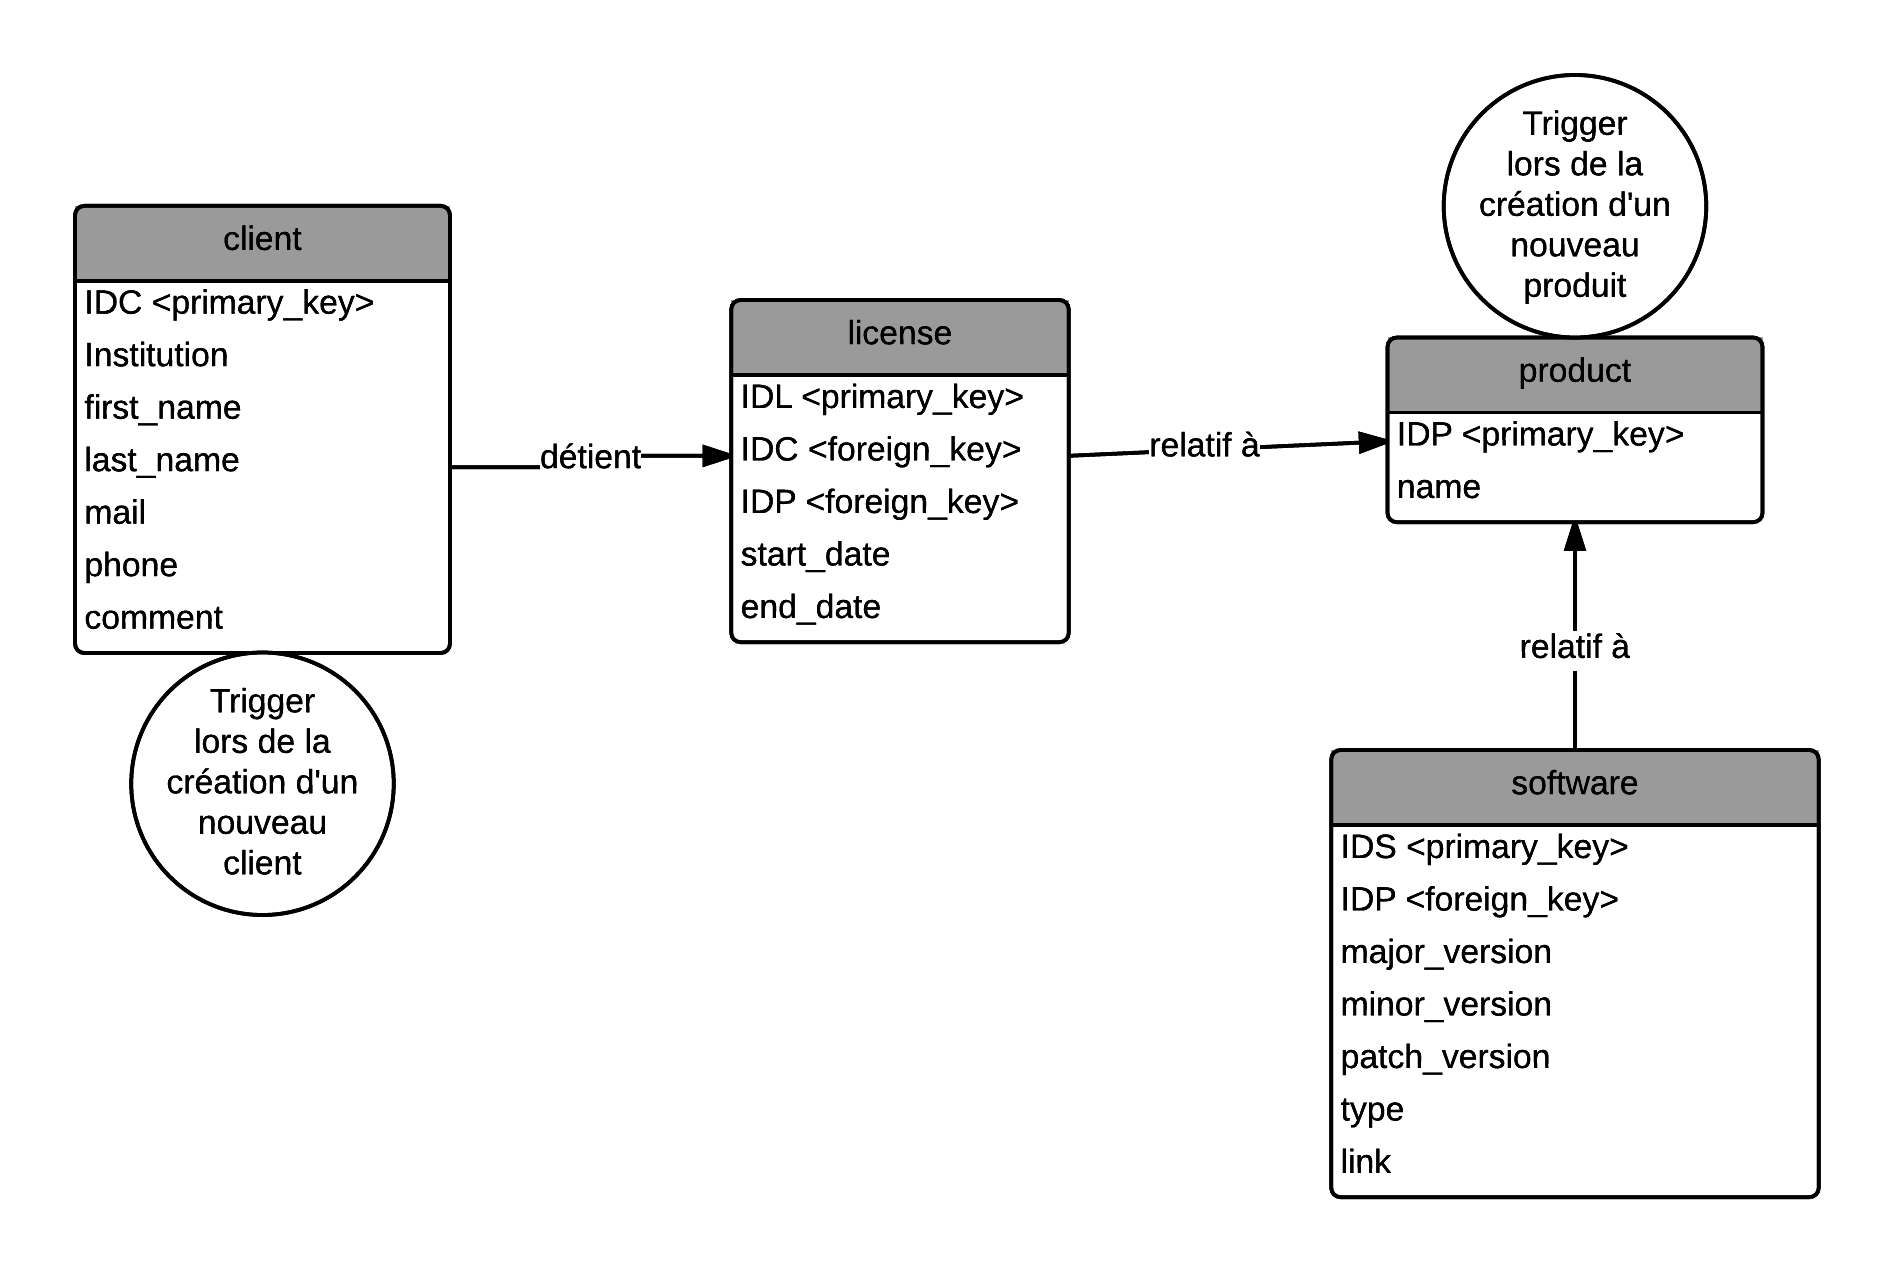
\includegraphics[scale=0.6]{images/MPD_sharokey.png}
\end{figure}
\end{frame}
\subsection{Conception dynamique et développement}
\begin{frame}
\frametitle{Composants de Sharokey}
\begin{figure}
\centering
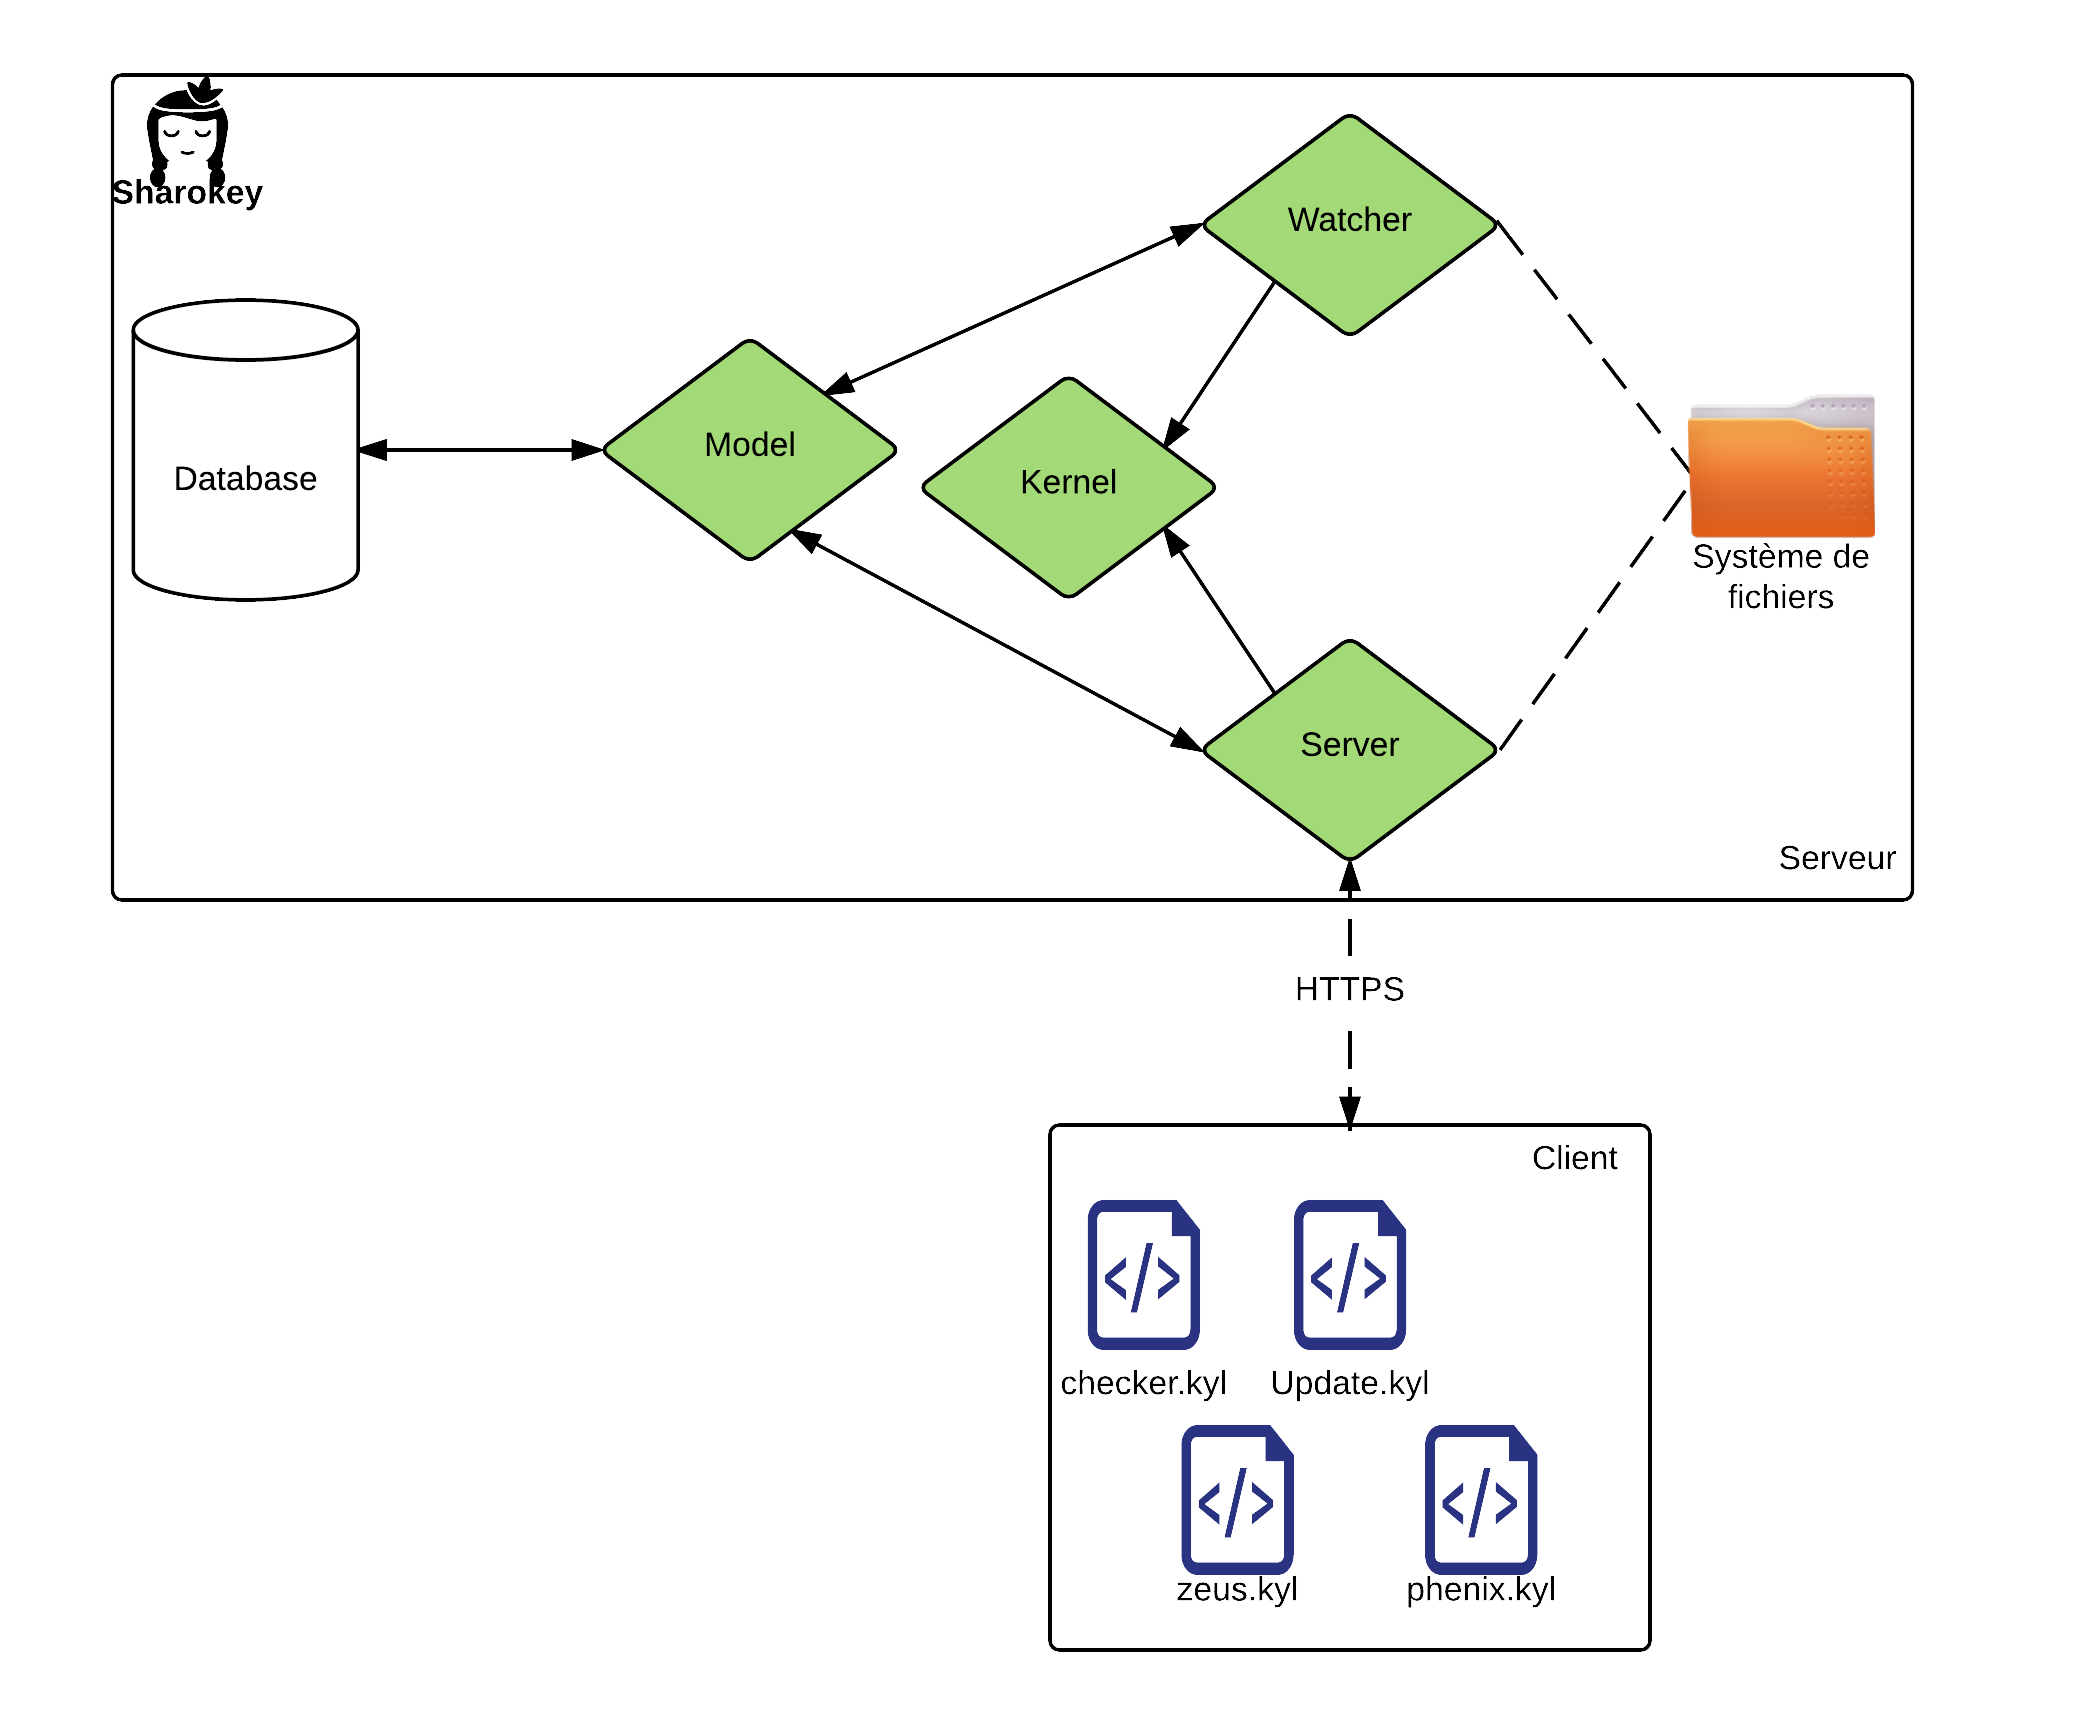
\includegraphics[scale=0.5]{images/composants.png}
\end{figure}
\end{frame}

\begin{frame}
\frametitle{Composants de Sharokey}
\begin{itemize}
\item Model : module NodeJS qui encapsule toute la logique liée aux opérations que les autres
composants peuvent effectuer sur la base de donnée. Ainsi, si un module veut effectuer
une opération sur la base de données, il devra passer par ce module.
\item Kernel : C’est le noyau NodeJS de Sharokey (l’API centrale) qui contient toutes les
fonctions communes aux autres modules.
\item Watcher : C’est le composant le plus dynamique du système il écoute les triggers de la base
de données effectue les modifications nécessaires sur le systèmes de fichier et vice-versa.
Il encapsule aussi la logique liée à la sécurité et la génération automatique et signature
des clés publiques et privés des nouveaux clients.
\item server : C’est le serveur NodeJS qui reçoit les requêtes des clients en HTTPS, vérifie la
signature sur leurs clés publiques, vérifie leur droit d’effectuer des mises à jour, prépare
et envoie la mise à jour sous format de scripts auto-extractible.

\end{itemize}
\end{frame}

\begin{frame}
\frametitle{Ajout d'un nouveau client}
\begin{figure}
\centering
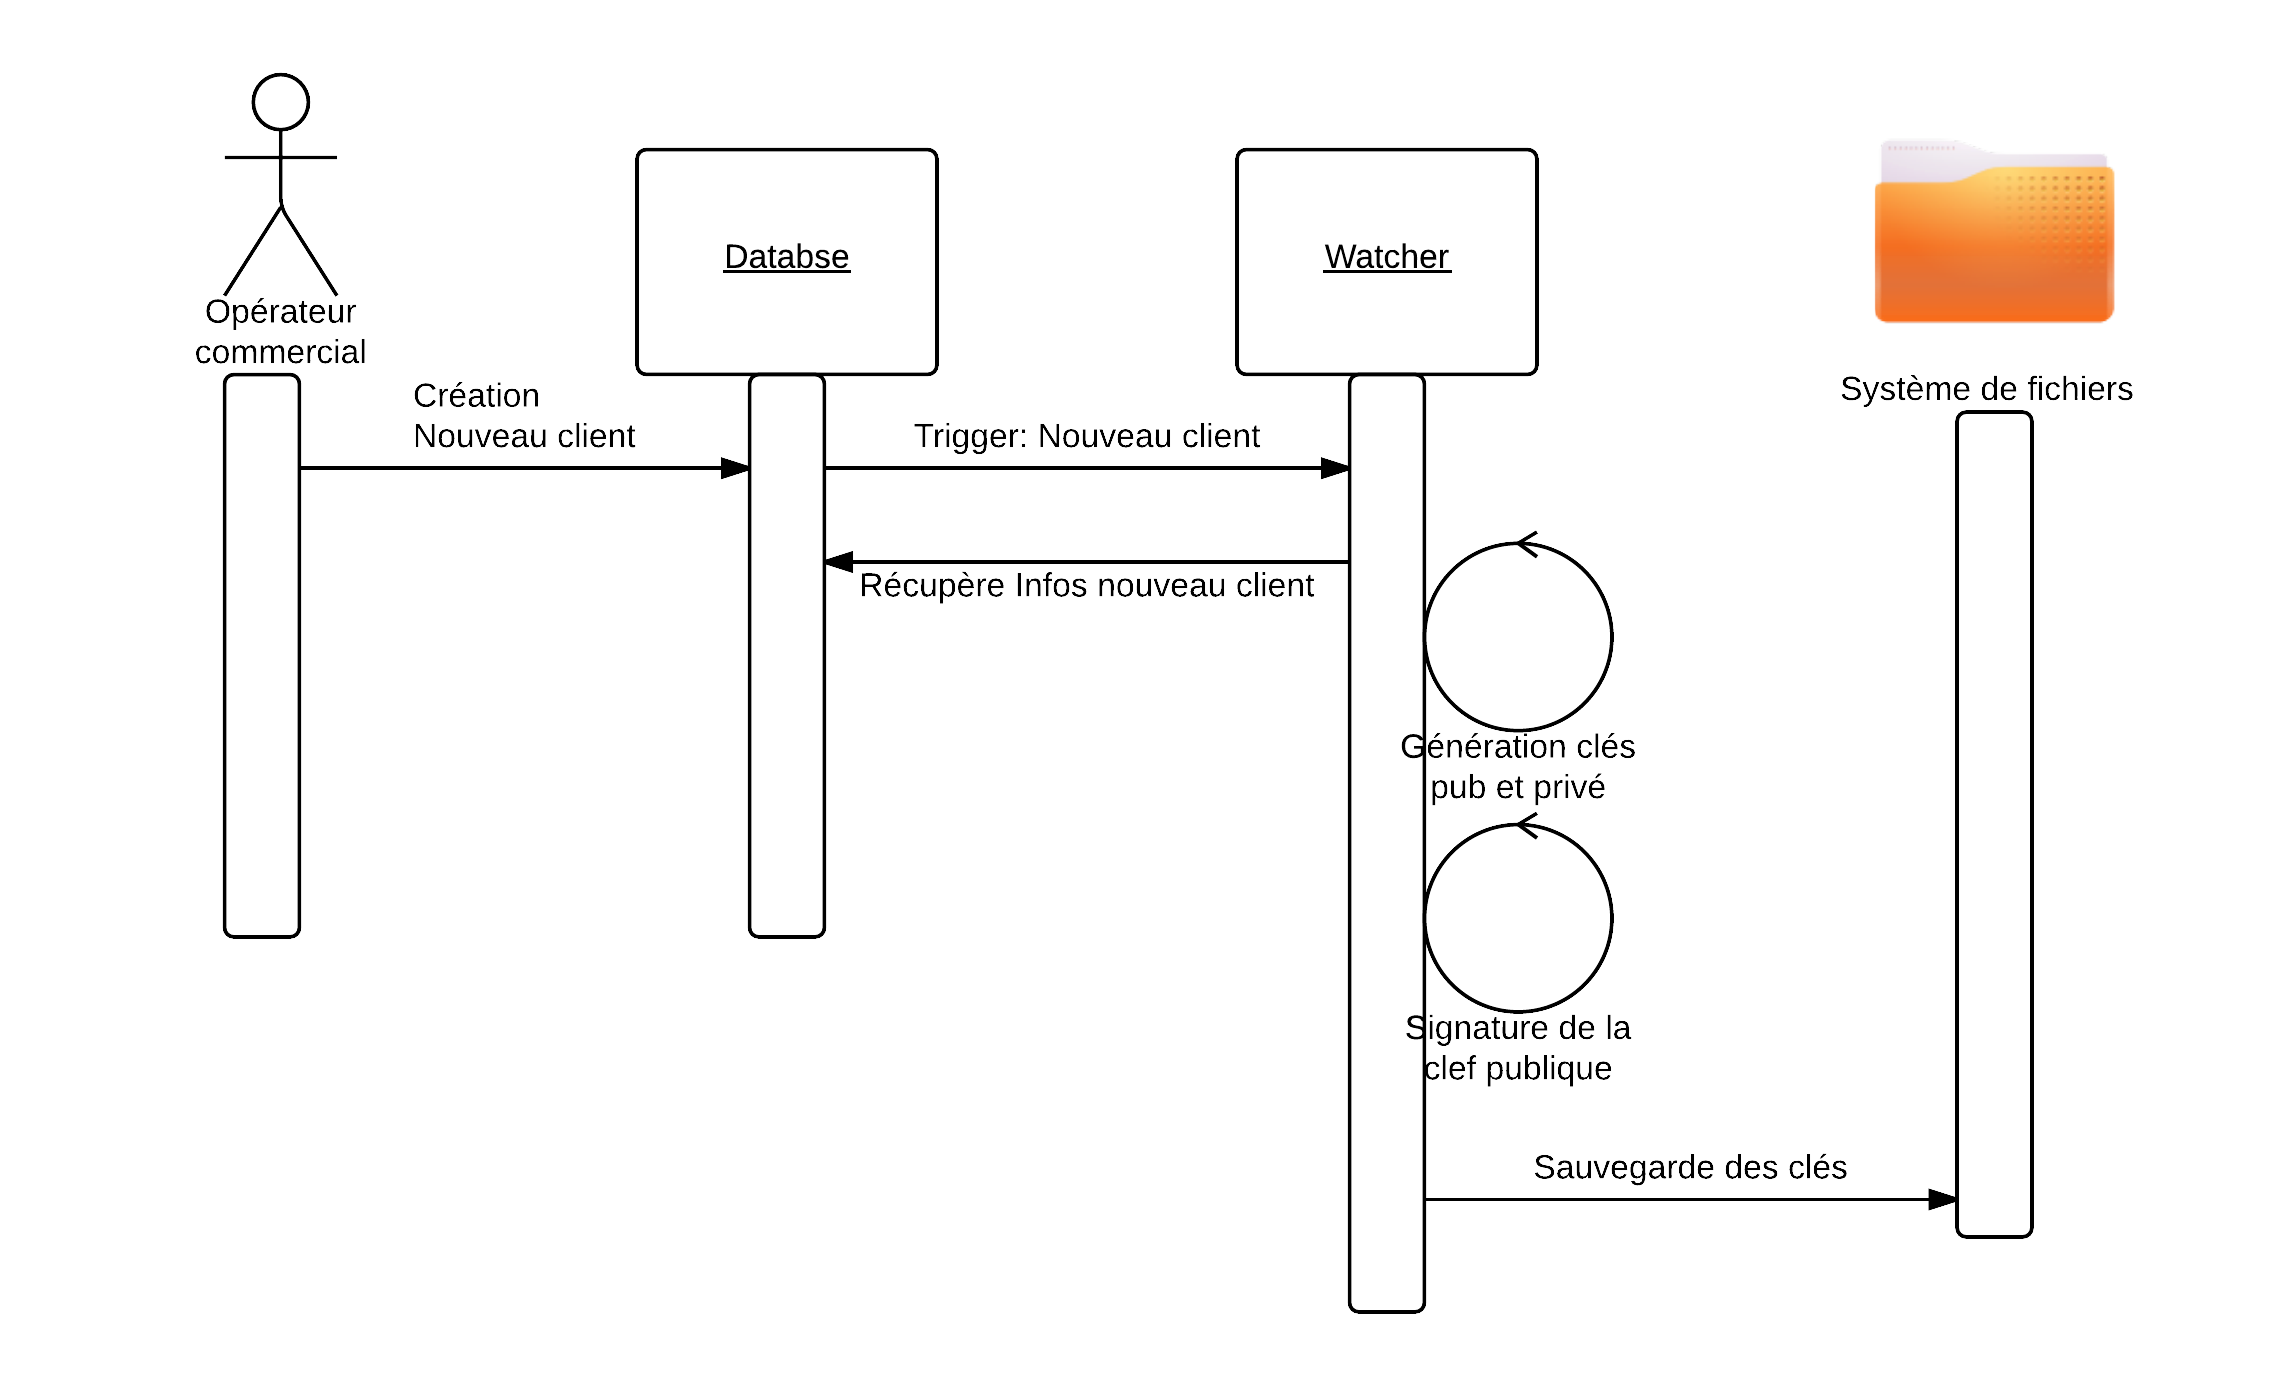
\includegraphics[scale=0.4]{images/1.png}
\end{figure}
\end{frame}

\section{Mise en place d'une infrastructure virtuelle de production des logiciels}
\begin{frame}
\frametitle{Production des logiciels}
\begin{figure}
\centering
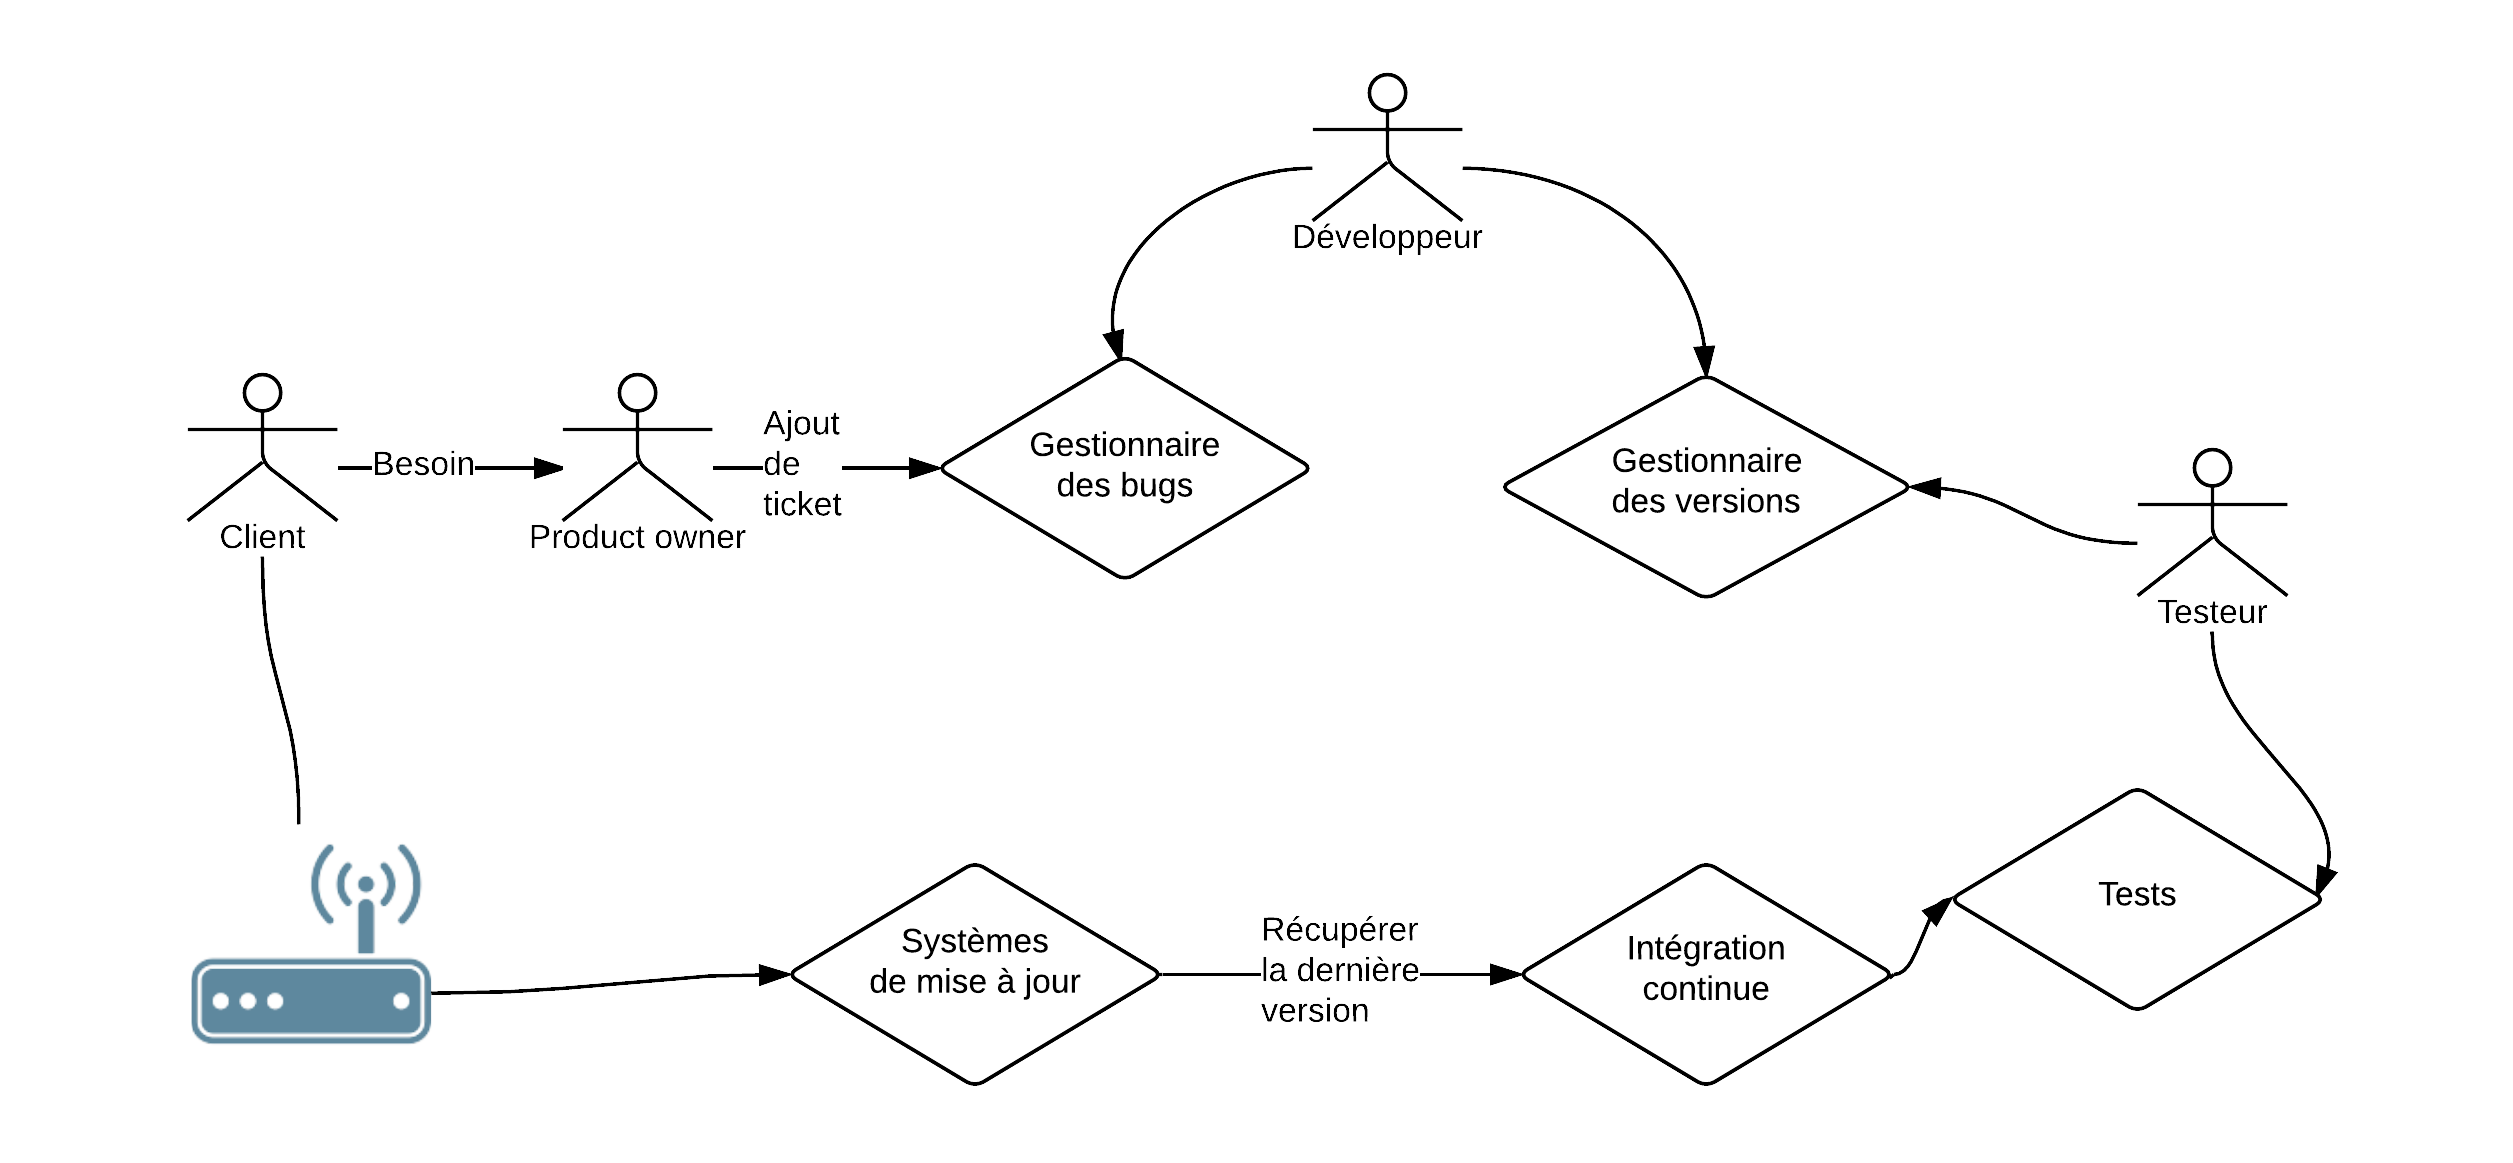
\includegraphics[scale=0.6]{images/fig3.png}
\end{figure}
\end{frame}

\begin{frame}
\frametitle{Production des logiciels}
\begin{figure}
\centering
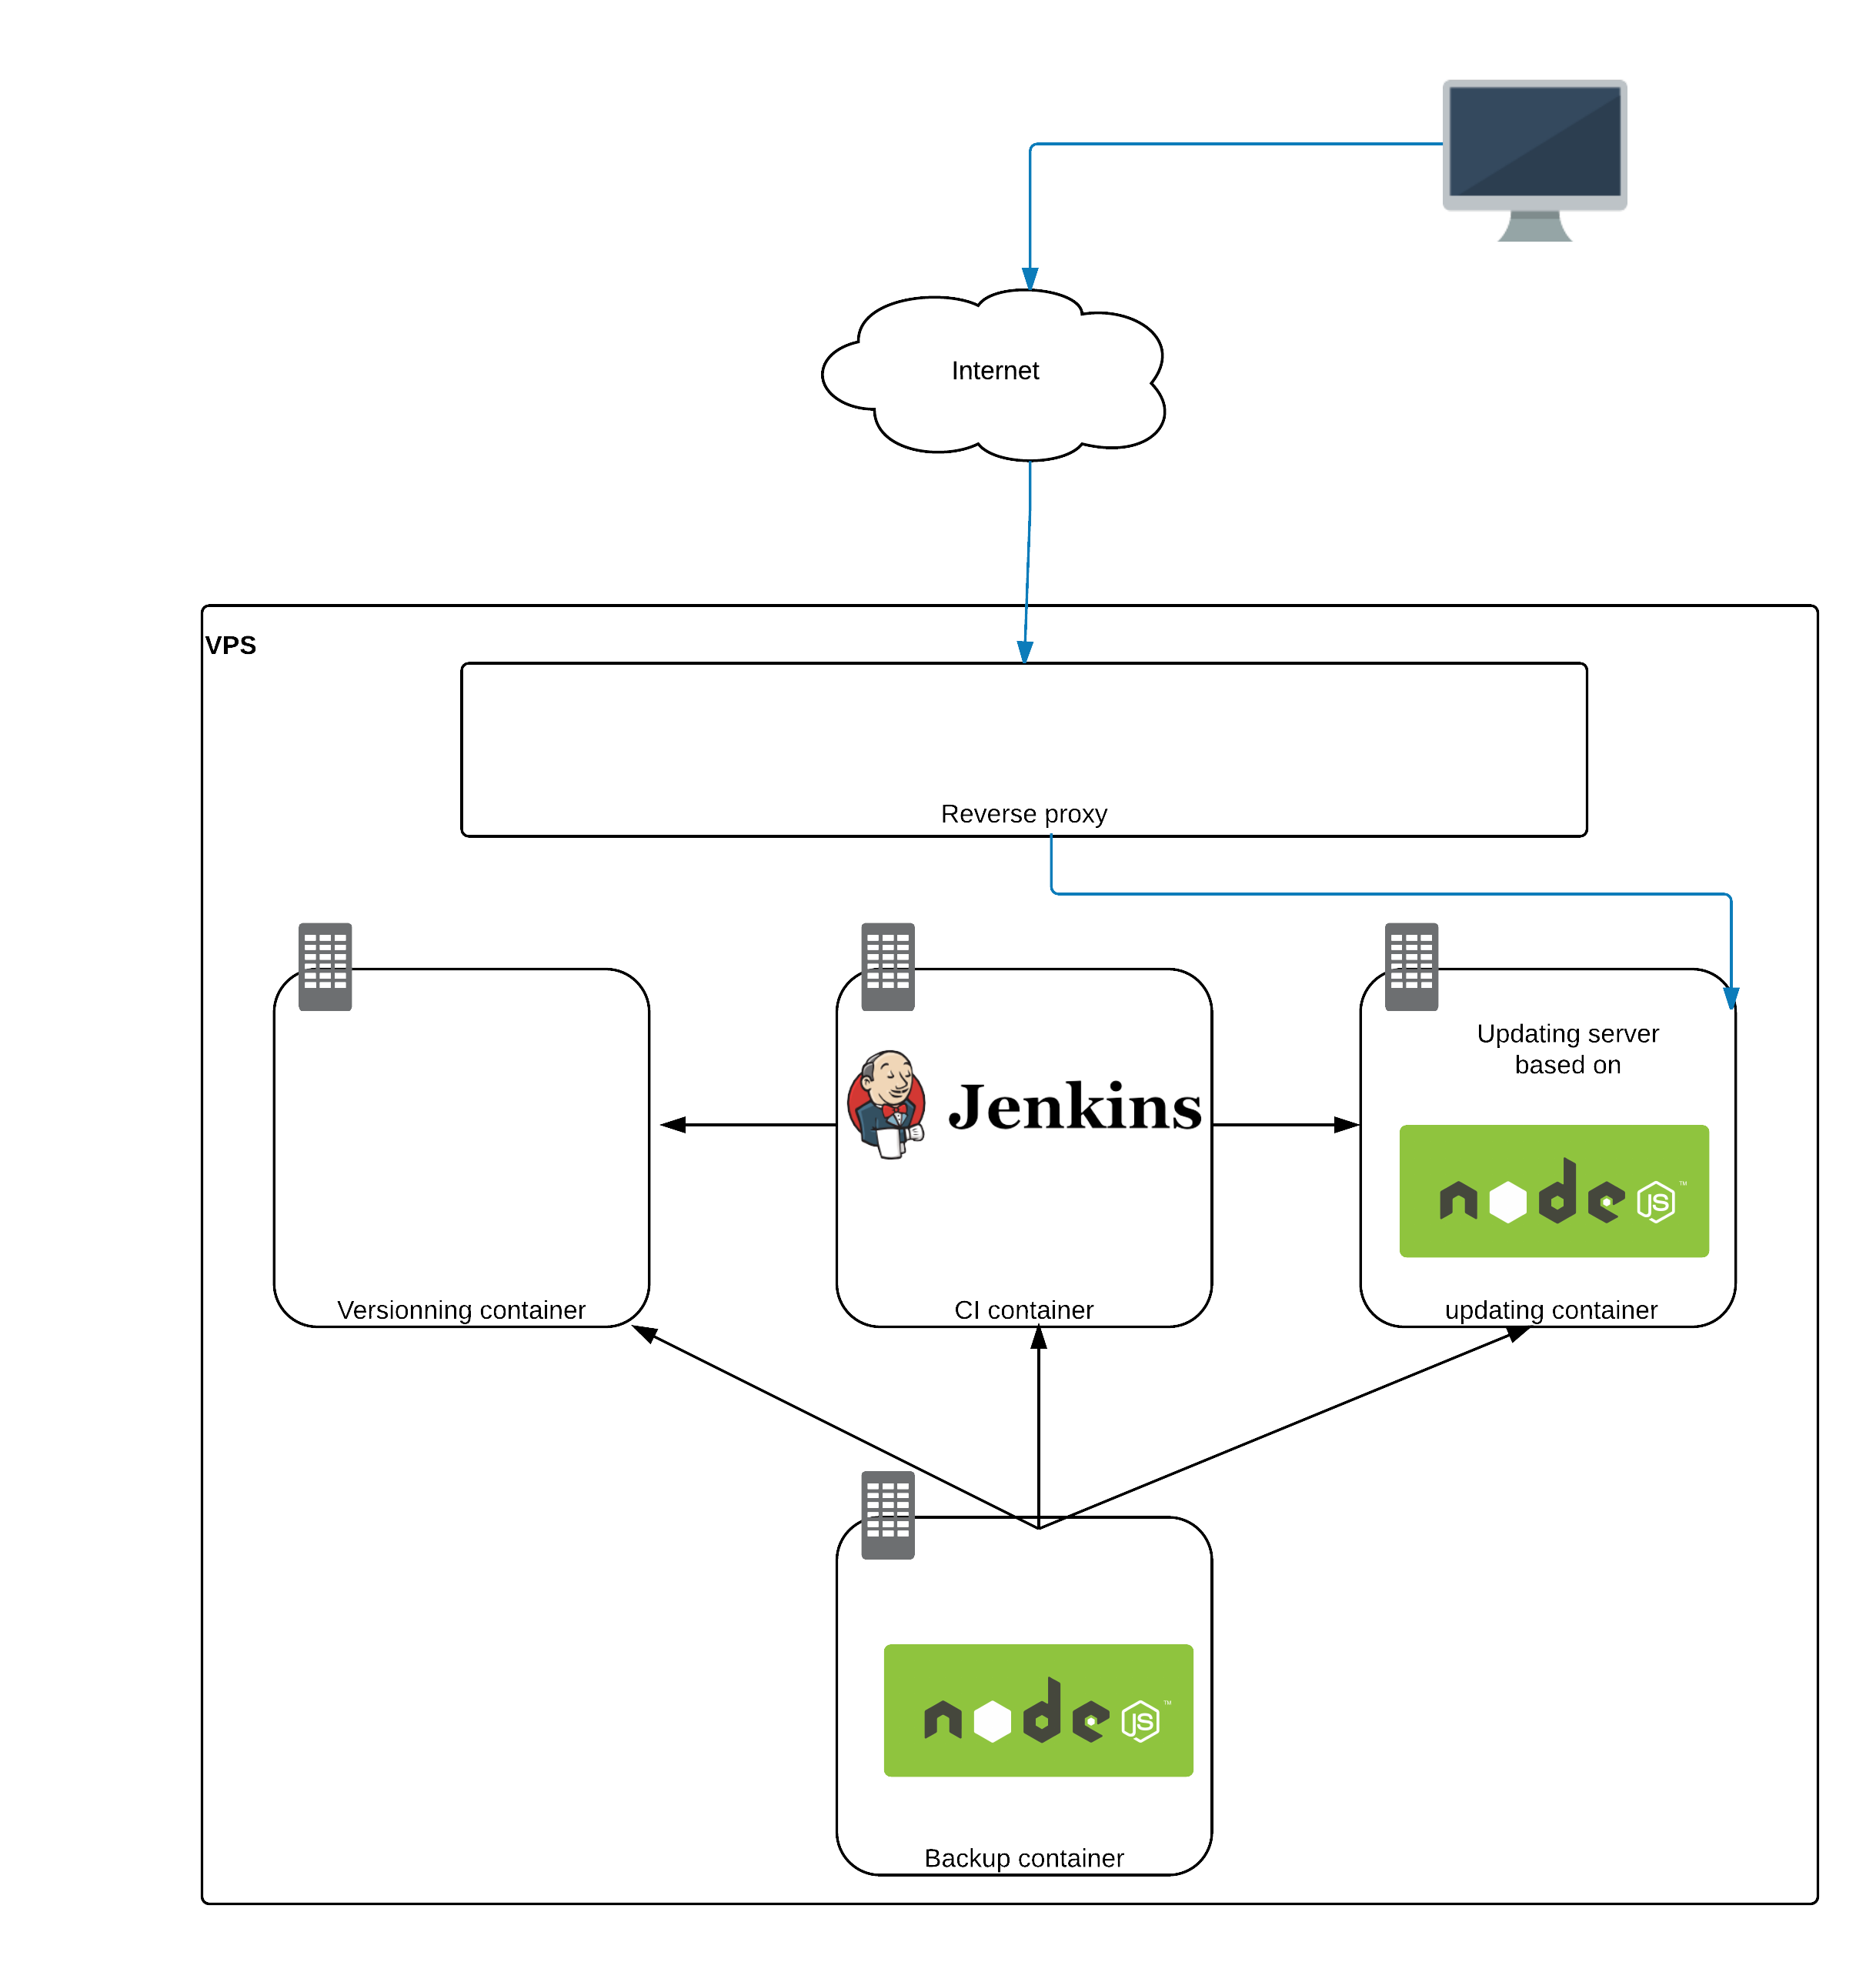
\includegraphics[scale=0.3]{images/vps1.png}
\end{figure}
\end{frame}

\section{Limites du travail}
%------------------------------------------------





%------------------------------------------------

\begin{frame}
\Huge{\centerline{Merci!}}
\end{frame}

%----------------------------------------------------------------------------------------

\end{document} 